%%This is a very basic article template.
%%There is just one section and two subsections.
\documentclass{article}

\usepackage{amsmath}
\usepackage{amscd}
\usepackage{amssymb}
\usepackage{amsfonts}
\usepackage{amsthm}
\usepackage{amsfonts}
\usepackage{amsthm}

\usepackage{circuitikz}
\usepackage{pgf}
\usepackage{tikz}
\usetikzlibrary{arrows,snakes,backgrounds}
% \usetikz
\usepackage{subfig}

\usepackage[super]{nth}
% \usepackage{appendix}
% \usepackage{listings}
% \usepackage{color}
\usepackage{ulem}
\usepackage{hyperref}
%\usepackage{url}
\usepackage{cancel}
\usepackage{cleveref}
 
\usepackage{aviolov_style}
\usepackage{local_style} 


\begin{document}


\title{Optimal Design for estimation in stochastic LIF models - \\ take 2} 
\author{Alexandre Iolov, Susanne Ditlevsen, Andr\'e Longtin  \\
$<$\href{mailto:aiolo040@uottawa.ca}
		{aiolo040 at uottawa dot ca}$>$, alongtin at uottawa dot ca}

\date{\today}

\maketitle

\abstract{Given a leaky, noisy integrate-and-fire neuronal model - we discuss
optimal design-type questions on what is the best external perturbation in order
to facilitate parameter estimation using discrete-time, trajectory observations}

\tableofcontents

\section{Problem Formulation}
The basic goal of 'Optimal Design' is to perturb a dynamical system in an
'optimal' way such as to 'best' estimate its structural parameters.

Consider the system 

\begin{equation}
dX = \underbrace{(\a + \b( \mu - X)}_{U(x,\a)} \intd{t} +
\underbrace{\s}_{\sqrt{2D}} dW
\label{eq:OU_evolution} 
\end{equation}

That can be solved as:
\begin{align*}
dX =& (\a + \b( \mu - X) dt + \s dW
% \\
% (dX + \b X_t) dt =& (\a + \b \m) dt + \s dW
\\
(e^{\b t} dX + e^{\b t}\b X_t) dt
=&
e^{ \b t}( \a + \b \m) dt + \s e^{\b t} dW
\\
Xe^{\b t} - X_0 =&
\int e^{ \b t}( \a + \b \m) dt +  \int \s e^{\b t} dW
\\
\implies
X_t =& e^{-\b t} X_0 
		+ \frac{(\a + \b \m)}\b \cdot ( 1- e^{-\b t}) +
	       \s  \cdot \sqrt\frac{{ 1 - e^{-2\b t}}}{2\b} \cdot \xi 
\end{align*}
where $\xi$ is a standard normal RV.

i.e. if $X_0$ is constant 
$$
X_t \sim N \left(e^{-\b t} x_0 + \frac{(\a + \b \m)}\b \cdot ( 1- e^{-\b t}),
\quad  \s  \cdot \sqrt{ \frac{ 1 - e^{-2\b t}}{2\b}} \right)
$$

Consider discrete observations ${X_n, t_n}$ obtained at uniform
$t_n$.
Then the transition probabilities $p_n(X_n|X_{n-1})$ are given by:
\begin{align*}
p_n(X_n|X_{n-1}; \m,\b, \s; \Delta_n) \propto &
\frac{\b}{\s \sqrt{1 -  e^{-2\b \Delta_n}}}
\\ &\cdot 
\exp\left(\frac{\left( X_n - (\frac \a\b + \mu)  - (X_{n-1} - \frac \a\b - \mu) \cdot
e^{-\b \Delta_n} \right)^2 \cdot \b}
			{ \s^2  (1-e^{-2\b\Delta_n})} \right)
\end{align*}
The likelihood is simply the product:
\begin{equation}
L( \{X_n\}| ; \m,\b, \s; \Delta_n; \a) = \prod_n p_n(X_n|X_{n-1}; \m,\b, \s;
\Delta_n)
\label{eq:Likelihood_OU}
\end{equation}
And the log-likelihood of  ${X_n, t_n}$ is
\begin{align*}
l(\b, \m, \s | )=& \sum \log p_n(X_n|X_{n-1})
\\
=& \frac{N}{2} \log \frac{\b}{\s^2(1-e^{-2\b\Delta_n})}
\\ & -\sum_n
{\left( X_n - (\frac \a\b + \mu)  - 
		(X_{n-1} - \frac \a\b - \mu) \cdot e^{-\b \Delta_n} \right)^2 } \cdot
				\frac{\b}{\s^2  (1-e^{-2\b\Delta_n})}
\end{align*}

\def \Xn {{ X_n }}
\def \Xm {{ X_{n-1} }}
\def \deltan {{ \Delta_n }}
% SAGE Derivation:
% \\
% In order to use classical formulas for ML estimates of OU  processes, we will
% rewrite $l$ in terms of the variable $$ m = \frac{\a + \b \m}{\b}$$
% which in the case of $\a=0$ gives $m=\m$.

ML estimators for $\m,\b,\s$ are obtained via setting $\di_{p} l$ to zero for
each parameter $p$. (ignore for now that $\Delta_n$ is not the same throughout).
However, it turns out that it is easier to first compute the ML estimate for
$\s$ and then plug it back into the likelihood, $l$, to simplify things:
\begin{align}
\di_{\s} l()=& -\frac N\s + 2\sum_n
\frac{ \left( X_n - e^{-\b \Delta_n} X_{n-1} -
				 (\frac \a\b + \m) \cdot ( 1-e^{-\b \Delta_n}) \right)^2 \b}
				 {\s^3 \cdot (1-e^{-2\b\Delta_n})}
				 \notag
				 \\ 
\implies \hat\s^2 =& 2\sum_n \frac{ \left( X_n - e^{-\hat\b \Delta_n} X_{n-1} -
				 (\frac {\a}{\hat{\b}} + \m) \cdot ( 1-e^{-\hat\b \Delta_n}) \right)^2
				 \hat\b} {N \cdot (1-e^{-2\hat\b\Delta_n})}
				 \label{eq:sigma_root}
\end{align}
With that the likelihood becomes:
\begin{align*}
l(\b, \m |\, X_n )=& 
 -N\log \left( 
 \frac{ \sum_n\left( X_n - e^{-\b \Delta_n} X_{n-1} -
  (\frac {{\a}}{{\b}} + \m) \cdot ( 1-e^{-\b \Delta_n})
  \right)^2}{N} \right) - 1
\end{align*}
Now maximizing the negative of a log plus a const is the same as minimizing the
argument of the log. So we need to {\itshape minimize}
\begin{align*}
l(\b, \m |\, X_n )\equiv& 
\sum_n \left( X_n - e^{-\b \Delta_n} X_{n-1} -
  (\frac {{\a}}{{\b}} + \m) \cdot ( 1-e^{-\b \Delta_n})
  \right)^2 
\end{align*}
% That is a non-linear least squares problem! And in fact it is bi-linear in the
% variable $$ b = \exp(-\b \Delta)$$ Billinear because of the term $\m b$.
 
Let's differentiate
\begin{subequations}
\begin{align}
\di_{\m} l()=& 2 \sum_n \left( X_n - e^{-\b \Delta_n} X_{n-1} -
  (\frac {{\a}}{{\b}} + \m) \cdot ( 1-e^{-\b \Delta_n})  \right) 
  \cdot   ( 1-e^{-\b \Delta_n})
\\
\di_{\b} l()=& 2 \sum_n \left( X_n - e^{-\b \Delta_n} X_{n-1} -
  (\frac {{\a}}{{\b}} + \m) \cdot ( 1-e^{-\b \Delta_n})  \right) 
  \\ \notag 
  & \times \left( \Delta_n e^{- \b \Delta_n}X_{n-1} 
  							  + \frac{ \a } {\b^2} (1-e^{-\b \Delta_n}) 
  					 		  - (\frac {{\a}}{{\b}} + \m) ( \Delta_n e^{- \b \Delta_n})          
  					 		  \right)
\end{align}
\end{subequations}
The $\m$ equation is straight-forward to solve

\begin{align}
\hat{\m} =&  \frac{ \sum_n \left( X_n - e^{-\b \Delta_n} X_{n-1} -
	\frac{\a}{\b} ( 1-e^{-\b \Delta_n}) \right)}
	{N ( 1-e^{-\b \Delta_n})}
	\label{eq:mu_root}
\end{align}

This means that we only need to solve one equation in one unknown
\begin{align}
\label{eq:beta_root}
0=& \sum_n \left( X_n - e^{-\b \Delta_n} X_{n-1} -
  (\frac {{\a}}{{\b}} + \m) \cdot ( 1-e^{-\b \Delta_n})  \right) 
  \\ \notag 
  & \times \left( \Delta_n e^{- \b \Delta_n}X_{n-1} 
  							  + \frac{ \a } {\b^2} (1-e^{-\b \Delta_n}) 
  					 		  - (\frac {{\a}}{{\b}} + \m) ( \Delta_n e^{- \b \Delta_n})          
  					 		  \right)
\end{align}
for $\b$ and then plug into \cref{eq:mu_root,eq:sigma_root}

(I have checked that in the case of $\a=0$ this reduces to well-known
expressions!)

Note: we've been quite cavalier about the constancy of $\Delta_n$, mostly
treating it as a constant, in order to focus on the impact of $\alpha$. Later we
can go back and be a little more rigorous, treating $\Delta_n$ as a function of
$n$.
 
On the contrary, while not being explicit in the notation, we have never assumed
$\a$ is constant and everything above can be rewritten in terms of $\a_n$.

\section{Optimal Design}
The ultimate question is how to choose the controls $\a(t) = \a(t_{n-1})$,
assumed piecewise constant over $\Delta_n$, such as to facilitate the estimation of the parameters
$\m,\b,\s$?

Two references suggest that one should use the mutual information
\cite{Myung2013,Lewi2009} as the criterion:

Let us follow \cite{Myung2013}:
Call the prior of the parameters, $\th = \{\m, \b, \s\}$:
$$\rho(\th)$$ and the posterior
\begin{equation}
p(\th| X; \a) =
\frac{L(x|\th; \a)\cdot \rho(\th)}{\int_\Theta L(x|\th; \a)\cdot \rho(\th)
\intd{\th}}
\label{eq:parameter_posterior_defn}
\end{equation} 
Where, $L$ is the likelihood of $X$ - $ L(X|\th; \a)$, that is given in
\cref{eq:Likelihood_OU}. $X$ could represent only one observation, $X_n$ or a
set of observations $\{X_k\}_n^{n+K}$.

Then one wants to optimize the mutual information:
\begin{equation}
I(\a) = \int_\Theta \int_X  \log\left[\frac{p(\th| x; \a)}{\rho(\th)}\right]
\cdot L(x| \th;\a) \cdot \rho(\th) \intd{\th} \intd{x}
\label{eq:mutual_info_objective}
\end{equation}
This is straight from equations 6,8,9 of \cite{Myung2013} (That paper is on
Mendeley)
 
Replacing the posterior in \cref{eq:mutual_info_objective}, with the bayesian
formula from \cref{eq:parameter_posterior_defn}, we get:
\begin{equation}
I(\a) = \int_\Theta \int_X  \log\left[\frac{L(x|\th; \a)}
										{\int_\Theta L(x|\th;\a)\cdot \rho(\th) \intd{\th}} \right] \cdot L(x|
										\th;\a) \cdot \rho(\th) \intd{\th} \intd{x}
\label{eq:mutual_info_objective_posteriored}
\end{equation}

We want to choose $\a$ as to make $I$ biggest. 

But now we need to consider how are we going to represent the parameter
distributions 
$\rho(\th) = \rho(\m,\b,\s)$???
And how are we going to update it\ldots?

One very simplistic way to proceed is take a Gaussian approximations for the
prior centred at the current ML estimates. Then to compute the argmax over $\a$
in \cref{eq:mutual_info_objective_posteriored}. But then to update the posterior using
the Gaussian approx'n / ML estimates again, instead of computing the true Bayesian
Update\ldots

This makes for a very nice soup - we have entropy (as the objective), Bayesian
updates (to form the entropy), ML likelihoods to center the estimates and Fisher
Information computation (evaluated at the estimates) to compute the Gaussian
Approximation (for the prior)\ldots:-)

So  
\begin{equation}
\rho(\th) \propto 
\exp\left( (\th - \hat\th) \cdot \hat\Xi^{-1} \cdot (\th-\hat\th)\right))
\label{eq:prior_gaussian_approxmn}
\end{equation}

Two questions:
\begin{enumerate}
 \item 
 How are we going to deal with the normalizing constant: ${\int_\Theta
 L(x|\th;\a)\cdot \rho(\th)}$?
\item How are we going to compute the Fisher Information? 
\end{enumerate}

There are two ways to compute the Fisher Info, $\FI$:
\begin{enumerate}
  \item As the covariance of the score $\FI = \Exp[ (\grad_\th l) :  (\grad_\th
  l)]$, this is the definition of $\FI$
  \item As the expected Hessian of the log-likelihood: $\FI = \Exp [ \grad
  \grad : l(\ldots)]$. This is only true, however, for the true parameters. 
\end{enumerate}

Hm! Maybe using Fisher Information for the Gaussian Approximation of
prior/posterior of the parameters is a BAD idea\ldots? 

More issues: in \cref{eq:mutual_info_objective} we have integration wrt.\ the RV
$x$. If, this is only one observation of the process, then 'x' is just $X_n$,
but if we take this to be $K$ observations: then 'x' is $\{X_k\}_n^{n+K}$ and we
have a $K$ dimensional integral\ldots However it does factor as we can
integrate, first wrt $X_n$ then $x_{n+1}$ and so on all the way to $X_{n+K}$.
% 
% I must say this is all quite painful.

One thing to do is for fixed $\th$ to sample a few $X$ paths. This is akin to
particle filtering\ldots then the objective will look like:

\begin{equation}
I(\a) = \int_\Theta \sum_{X_i|\th}  \log\left[\frac{L(X_i|\th; \a)}
										{\int_\Theta L(X_i|\th;\a)\cdot \rho(\th)\intd{\th}} \right]
										 \cdot \rho(\th) \intd{\th}
\label{eq:mutual_info_objective_particlized}
\end{equation}

Now suppose that $\th$ is chosen using some kind of a Gauss-Hermite quadrature
scheme in 3-d. Say that requires 125 points (that is only five points in each
direction, so quite conservative, but also should be quite efficient!) That
means that to evaluate $J$ we need to sample $I \times 125$ paths. And then do
the summation. But wait, there's more. For each $x,\th$ pair we also need to do
the integral for the normalizing constant\ldots so now we have $I \times 125^2$
calculations. Just to evaluate $J$.

Uf! 

Still that is what we have computers for\ldots But there should be something
simpler to do\ldots 

\subsection{Simple illustration}
Let us make a simple proof-of-concept.

We will take for the true parameters
$$
\b = .05; \m = -60; \s = .1;
$$
Now since the values of $\m, \s$ are determined by $\b$, let us reduce the prior
to a one-dimensional Gaussian
$\rho(\b) \propto \exp( -(\b -\hat \b)^2 / {\s_\b}^2) $
and then for a given $\b$ we will obtain $\m, \s$ from
the formulas in \cref{eq:mu_root,eq:sigma_root}.

We will only focus on the next observation, so the likelihood is also a gaussian
distribution (conditional on $\m,\b,\s$) in 1-d. 

Let us write it out using $x_0$ as the current value and $x$ as the future
value and $\Delta$ as the time interval until the next observation:
then the terms $L,\rho$ in the mutual information
\begin{align*}
I(\a) =& \int_\Theta \int_X  \log\left[\frac{L(x|\th; \a)}
										{\int_\Theta L(x|\th;\a)\cdot \rho(\th) \intd{\th}} \right] \cdot L(x|
										\th;\a) \cdot \rho(\th) \intd{\th} \intd{x}
										\end{align*}
										are given by:
\begin{align*}
L(x|\th; \a) =& \frac{\b}{\s \sqrt{2\pi(1 -  e^{-2\b \Delta}})}
 	\cdot \exp\left(\frac{\left( x - (\frac \a\b + \mu)  - (x_{0} - \frac \a\b
 	- \mu) \cdot e^{-\b \Delta} \right)^2 \cdot \b} { \s^2  (1-e^{-2\b\Delta})}
 	\right) 
 	\\
 	\rho(\th) =&  
 	\frac{1}{\s_\b \sqrt{2\pi} } \exp(-\frac{(\b-\hat\b)^2}{\s_\b^2}) 
		\end{align*}
Thus for each $x$ we need to form a Gaussian integral for the normalizing
constant. And on top of that we need to make a two dimensional independent
gaussian integral for the $x,\b$.

Let us illustrate this. For the calculations we will use 1. Gauss-Hermite
integration and 2. simple Curtis-Clenshaw integration as a sanity check. 

Let us start with a sample of 50 (ms) observations sampled at .1 ms. Then if we
take a coarser sampling of 1s to create our boot-strap of estimates for $\beta$
we get:
\begin{equation*}
\begin{gathered}
\hat \beta \quad \s_{\hat\b} \\
0.0881, 0.0182\\
0.0974, 0.0514\\
\boxed{0.0902, 0.0562} // \textrm{used in subsequent simulations}\\
0.3060, 0.2968\\
0.0696, 0.0386\\
0.1947, 0.0790\\
0.1702, 0.0624\\
0.1706, 0.0481  // \textrm{way off including too small std}\\
 0.1332, 0.0879\\
\end{gathered}
\end{equation*}
That is actually ok. In 1 case, we couldn't actually estimate $\b$ (the data
implies there is no solution to \cref{eq:beta_root}). In the other 9 cases, 8
times the true value (.05) is within 2 standard deviations of the mean estimate
and in 5 cases it is within 1 standard deviation of the mean.

Note that calculating $\s_\b$ as $$ \s_\b^2 = \sum(\hat{ \hat \b} - \hat \b)^2
$$ where $\hat{ \hat \b}$ are bootstrap estimates from a reduced data set helps
increase the value of $\s_\b^2$. If instead of $\hat \b$, we use the mean of the
bootstrap values themselves to calculate $\s_\b$, we will get smaller values for
$\s_\b$, which will usually put the true value more than two standard deviations
from the short-time estimate.

Let's use the values of $\hat \beta, \s_{\hat\b} =  0.0902, 0.0562$ and
visualize the resulting distributions for $\b$ and the functions $\m(\b),
\s(\b, \m)$, see \cref{fig:prior_mu_sigma}. Essentially what we see is that $\m$
depends on $\b$ inversely while $\s$ does not really depend on $\b$ given the
data and a $\m$ estimate. That is perfectly natural. We know that the long term
equilibrium of $X_t$ is $\m\b$, so given a sample, $\hat \m$ will be roughly
equal to the sample mean divided by $\hat \b$. On the other hand $\hat \sigma$
seems affected only by the product $\hat \m \hat \b$, so that for a given $\b$,
once $\m$ is estimated the two variations cancel each other and we get the flat
line on the bottom panel in \cref{fig:prior}.
\begin{figure}[h]
\begin{center}
\subfloat[prior]
{
\label{fig:prior}
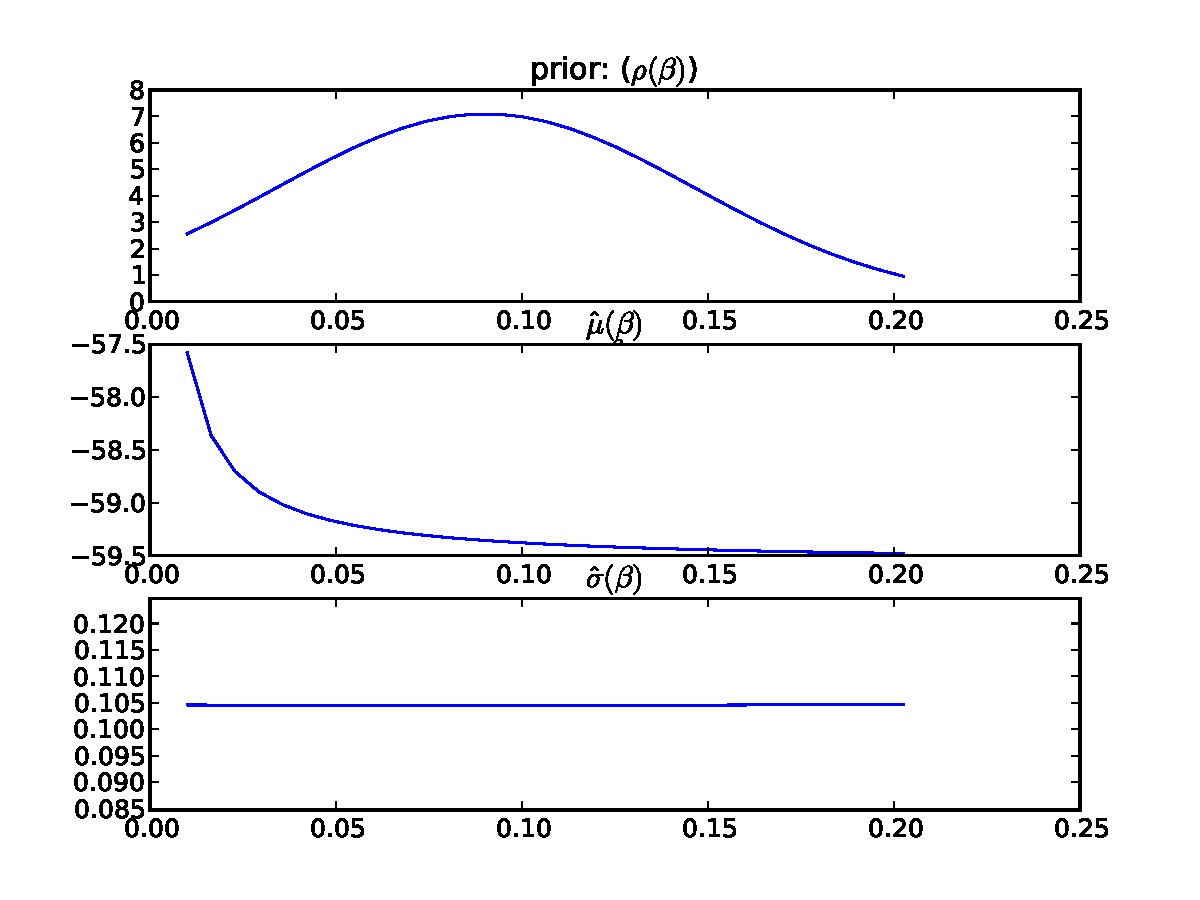
\includegraphics[width=0.48\textwidth]{Figs/MI/prior_example.pdf}
}
\subfloat[underlying $X$ path]
{
\label{fig:prior_path}
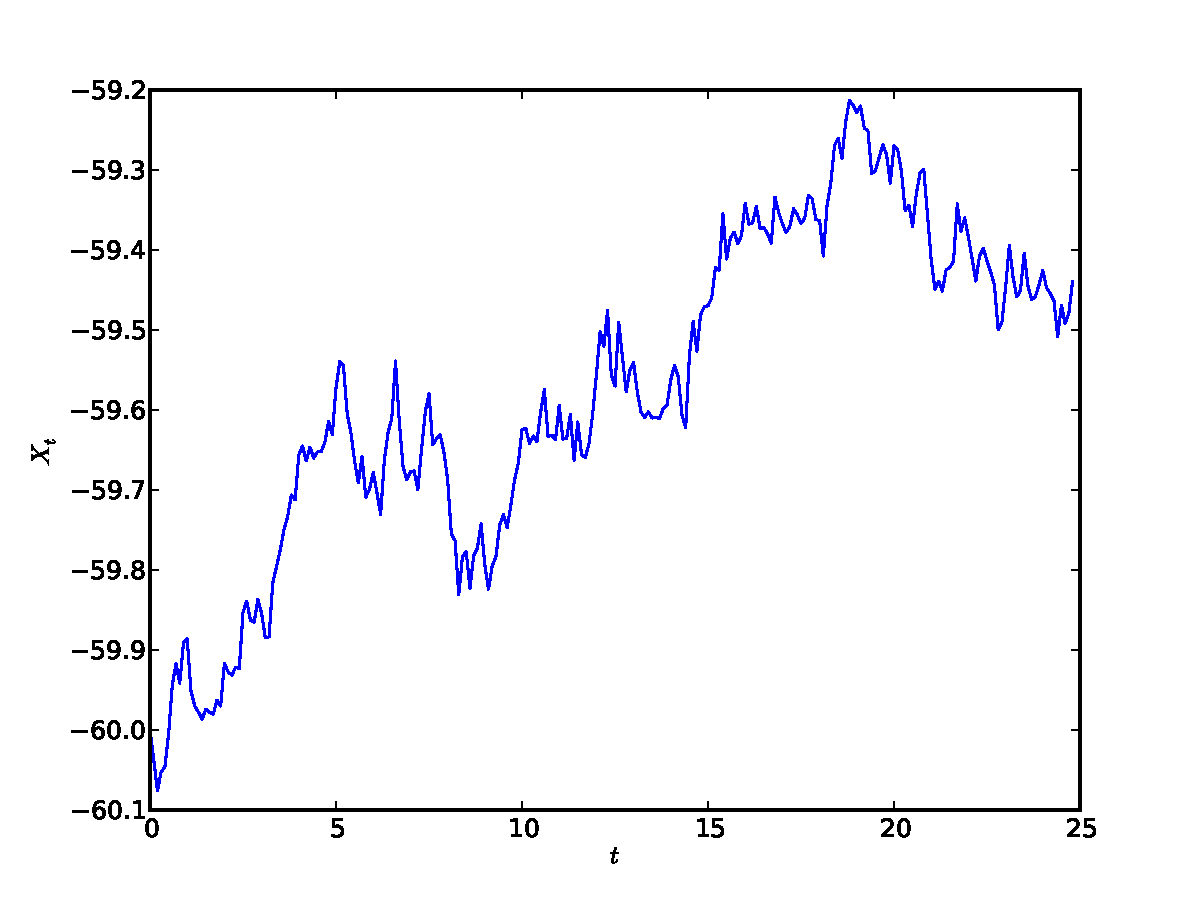
\includegraphics[width=0.48\textwidth]
{Figs/MI/prior_example_path.pdf}
}
\caption[labelInTOC]{An example of a path, a prior over $\b$ built based on
the path and the resulting functional relations between $\b$, $\m$ and $\s$,
which are from \cref{eq:mu_root,eq:sigma_root}. The prior for $\b$ and the
resulting $\m,\s$ are obtained using the path in (b)}
\label{fig:prior_mu_sigma}
\end{center}
\end{figure}
At this point we might start to think a normal prior for a positive random
variable is a bad idea, especially if we are near zero and the std. dev. is
non-negligible. Perhaps, we should use a log-normal prior or a gamma
distribution \ldots


Now let's calculate the integral of the likelihood wrt.\ the prior for a fixed
$x$, ie. the marginal forward distribution of $x$. $$ p(x) = \int_\Theta
L(x|\th;\a)\cdot \rho(\th) \intd{\th} $$ This is also the normalizing constant
in bayes rule. We will used a forward horizon of  $\Delta_f = 5$ (ms) (For
reference, the data has $\Delta = 0.1$ and has length $T = 50$ ms). $p(x)$ si
shown in \cref{fig:marginal_px}. Essentially, \cref{fig:marginal_px} is telling
us that the current value of $x$ is unlikely, all things considered. Our current
estimates for $\b, \m, \s$ are letting us believe that it should be
significantly closer to $59.5$ if we continue with the current value of $\a=0$.
The two opposing proposed values for $\a = \pm 0.25$ result in much more spread
distributions for $X_{t+\Delta_f}$. In particular, one might argue that
$\a=-0.25$ is most informative, since the forward distribution has the most
spread. (if we intuitively equate spread with information). This is consistent
with the notion that the most informative experiments are the ones that lead $X$
furthest from its current equilibrium (given $\a=0$). In this case the negative
is better than positive, since the current value of $X_t$ is already negative in
relation to the current equilibrium. Basically this is consistent with the
following selection mechanism of $\a$: If $X_t > \m \b$ choose $\amax$ otherwise
if $X_t < \m \b$ chose $\amin$. This is illustrated in
\cref{fig:marginal_px_shifted}, where we artificially move the value of $X_t$ to
the right of the (current) equilibirum, which makes the forward distribution
arising from $\a=0.25$ more informative (higher spread), then the one with
$\a=-0.25$
% \usepackage{graphics} is needed for \includegraphics
\begin{figure}[htp]
\begin{center}
\subfloat[Left of equilibrium]{
  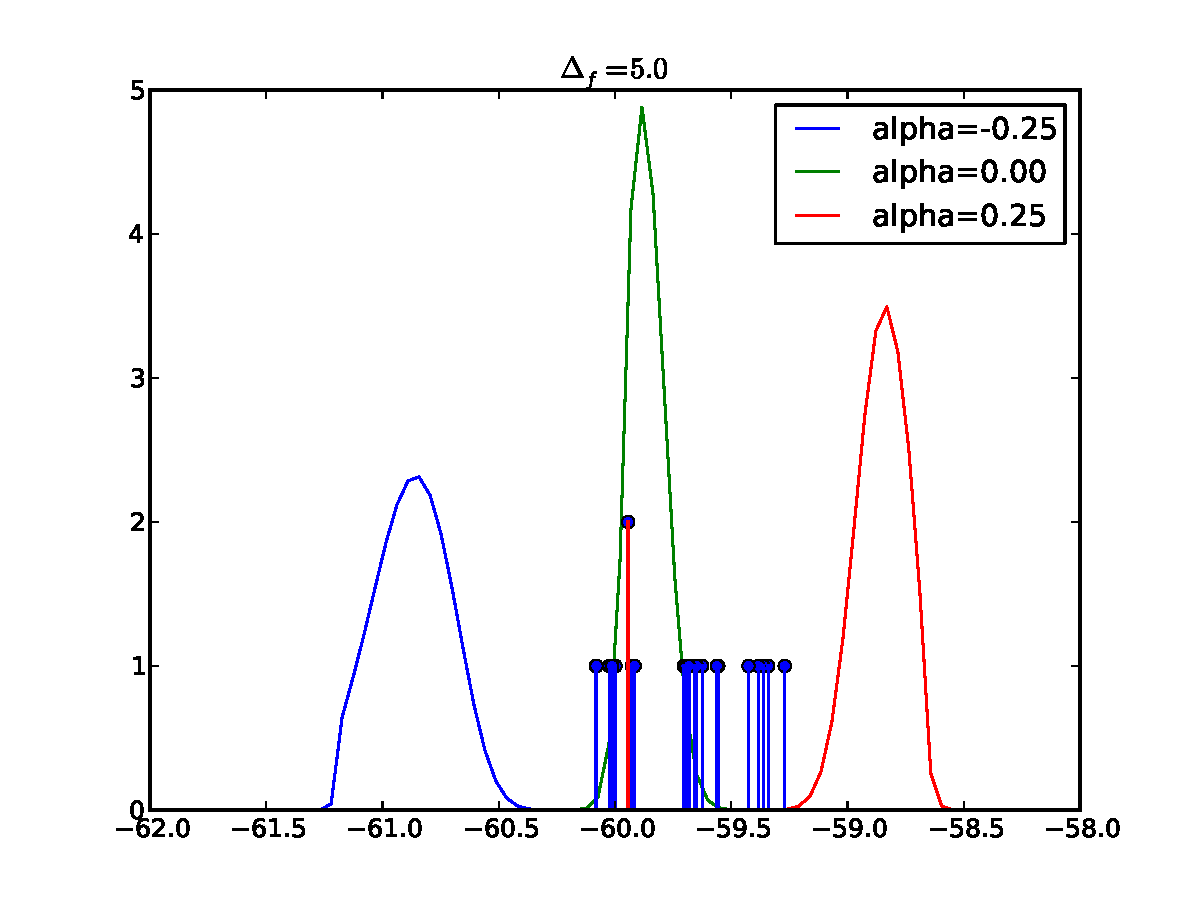
\includegraphics[width=.5\textwidth]{Figs/MI/x_marginal_example.pdf}
  \label{fig:marginal_px}
}
\subfloat[Right of equilibrium]{
  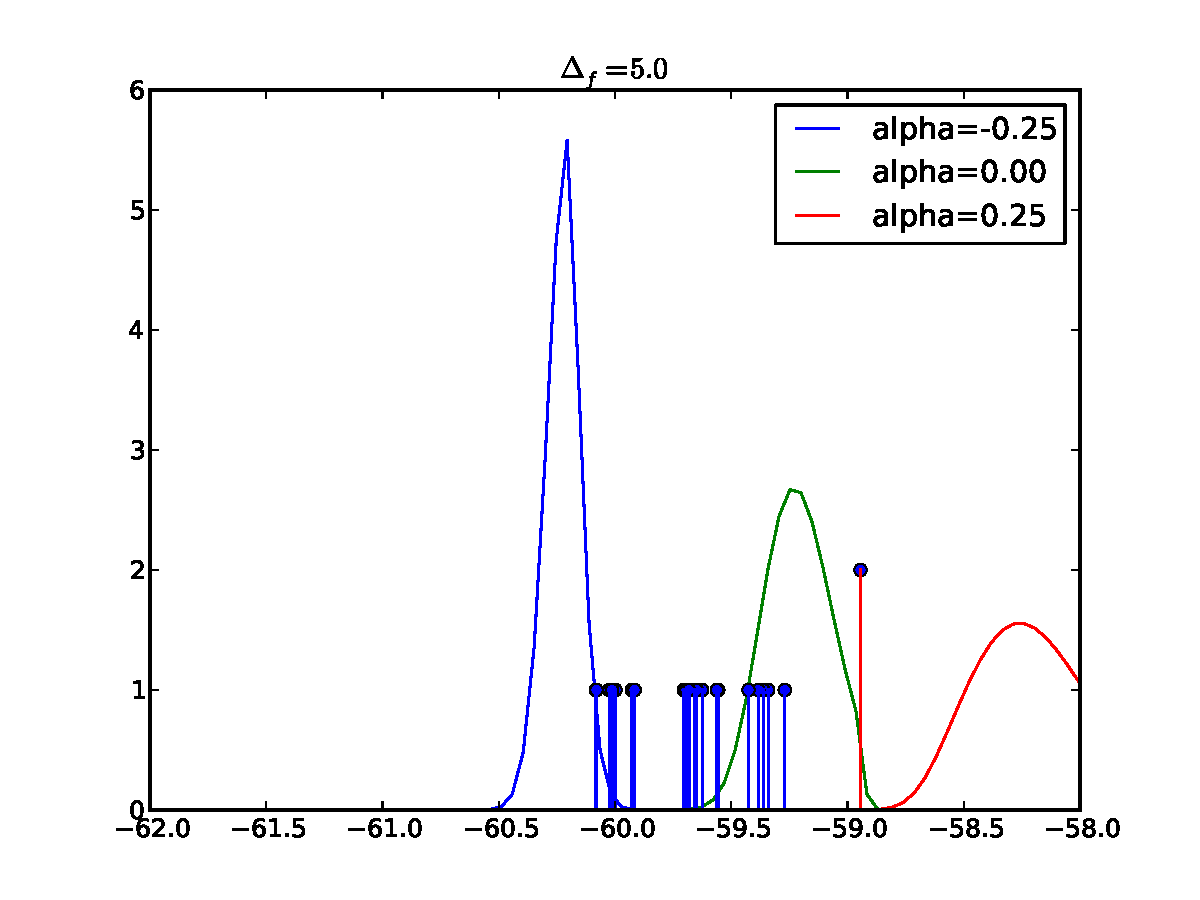
\includegraphics[width=.5\textwidth]{Figs/MI/x_marginal_example_x0_shifted_right.pdf}
    \label{fig:marginal_px_shifted}
  }
  \caption[labelInTOC]{
  Marginal of $x$ (normalizing constant), the tall red stem
  is the current value of $X_t$. This is the last observed value based on
  which we compute transition densities. The blue and red curves are forward densities
  given different applied forward values for $\a$. The green curve is the
  forward density given the hitherto used value of $\a=0$. It mostly coincides
  with the so-far observed data which is the blue stems.
  In float (b) we artificially move the starting point to the right. Note that
  the green curves in a), b) are not the same, since they depend on the value
  of $x_0$ as well as the observed data (which is the same in both panels)}
\end{center}
\end{figure}

Let us verify this intuition formally, by calculating $I(\a)$, for $\a =[-0.25 , 0, 0.25]$.

An aside: Unfortunately, naively calculating the double integral (in Python
using 'quad' or 'romberg') is not numerically efficient. Calculating $I(\a)$ for a single
$\a$ takes on the order of 10 secs, once you relax the quadrature
tolerances without incurring any significant error\ldots On the other hand the process is supposed to be taking on the order of milliseconds. We need to be
NOT naive! Since we are dealing with Gaussian-type integrals, a Gauss-Hermite
Integration scheme might be very effective\ldots But let's leave that for now.

Now, crushing through with brute force we get the result
in \cref{tab:MI_3alphas_basic_quad}.
\begin{table}
\begin{centering}
\begin{tabular}{cc}
$\a$& $I(\a)$ \\
-0.25  &
 0.688 
\\
0.00 &
   0.100 
\\
   0.25 &
   0.419 
\end{tabular}
\caption{values of MI}
\label{tab:MI_3alphas_basic_quad}
\end{centering}
\end{table}
We have used the same starting (current) value of $X_t$ to form the forward
likelihoods as in \cref{fig:marginal_px} and indeed we get the result.
$$I(-0.25) >I (.25) > I(.0)$$
which is consistent with our expectations after calculating the corresponding
$p(x)|\a$ in \cref{fig:marginal_px}. This basically says that it should be most
informative to stimulate down ($\a<0$), and it should be least informative to
do nothing $\a=0$.

 \subsection{Experiment}
 Let's now see what that means in practice. We will pretend that we have done the
 analysis in a blink and then see what happens when we further simulate the
 process from $X_t$ for $\Delta_f$ time and see if there is any advantage to
 using the mutually most informative $\a$, i.e.\ $\a = \argmax I(\a)$, or not. 
% 
First we generate 10 forward trajectories of duration 2$\Delta_f = 10$ (ms).
They are shown in \cref{fig:perturbed_trajectories}.
\begin{figure}[htp]
\begin{center}
  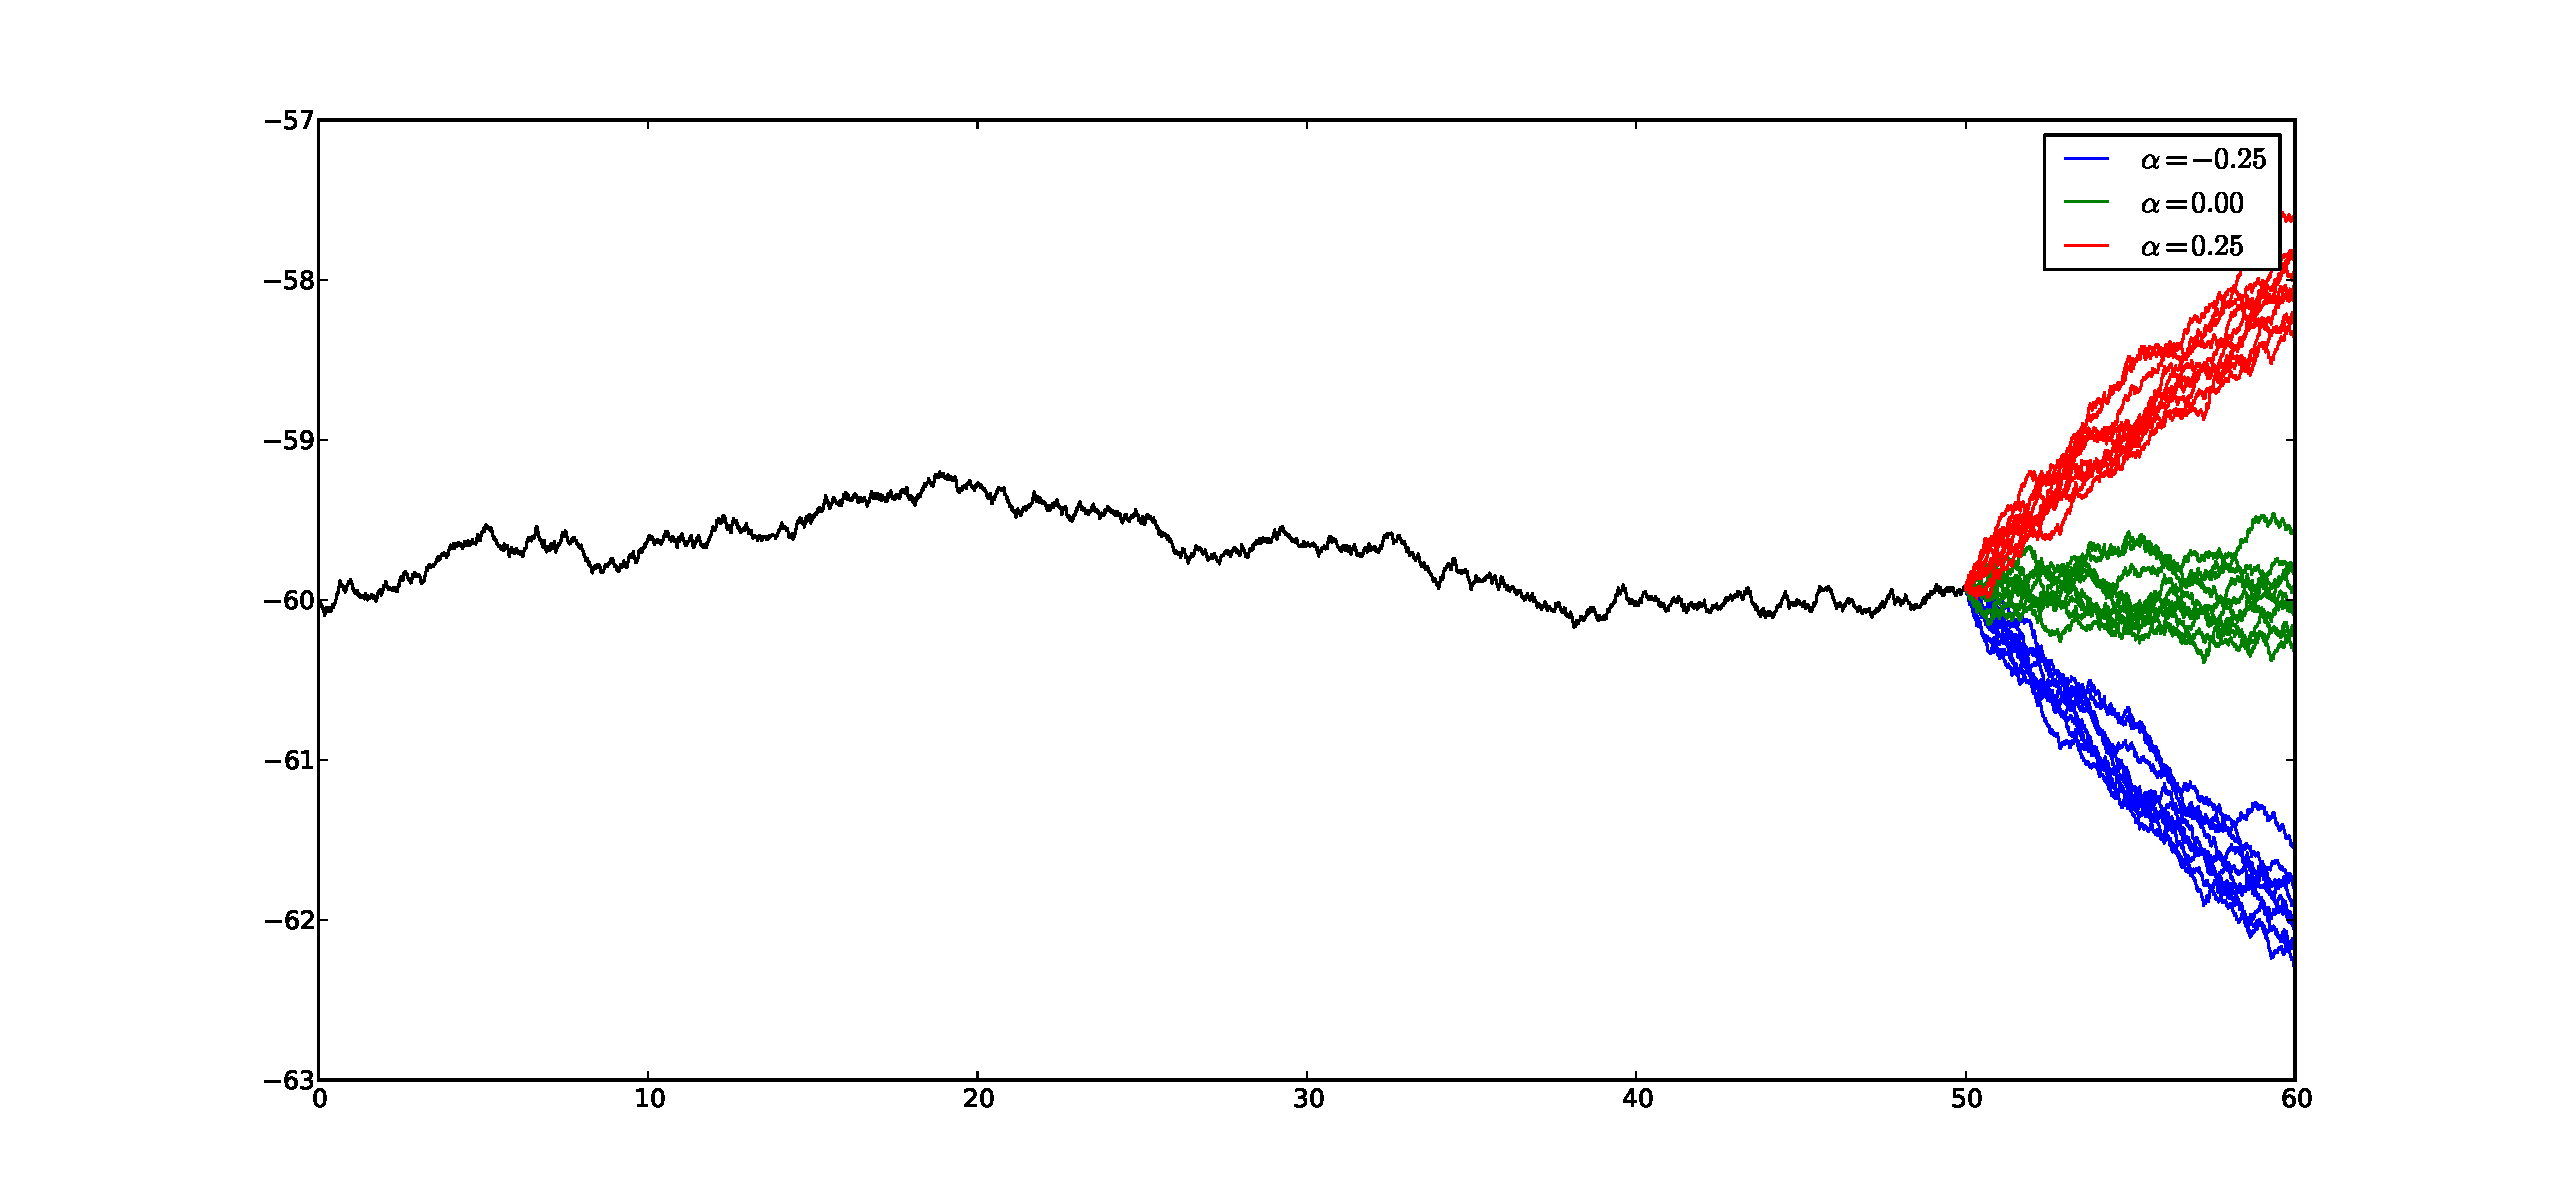
\includegraphics[width=1\textwidth]{Figs/MIML/forward_sims.pdf}
  \caption[labelInTOC]{Different Trajectories perturbed by different values of
  $\a$ after the MI calculation}
  \label{fig:perturbed_trajectories}
\end{center}
\end{figure}
% 
Now what we would like to see is that the estimates corresponding to $\a=-.25$
are 'better' than the ones corresponding to $\a=.25$ and that they are much
better than the ones corresponding to $\a=.0$.

Let's see: The resulting estimates for the 10 trajectories are shown in
\cref{fig:perturbed_estimates}. Well, what do you know, visually, it is clear
that indeed $\a=-.25$ is  'better' than $\a=.25$, which in turn is better than $\a=.0$.
\begin{figure}
\begin{center}
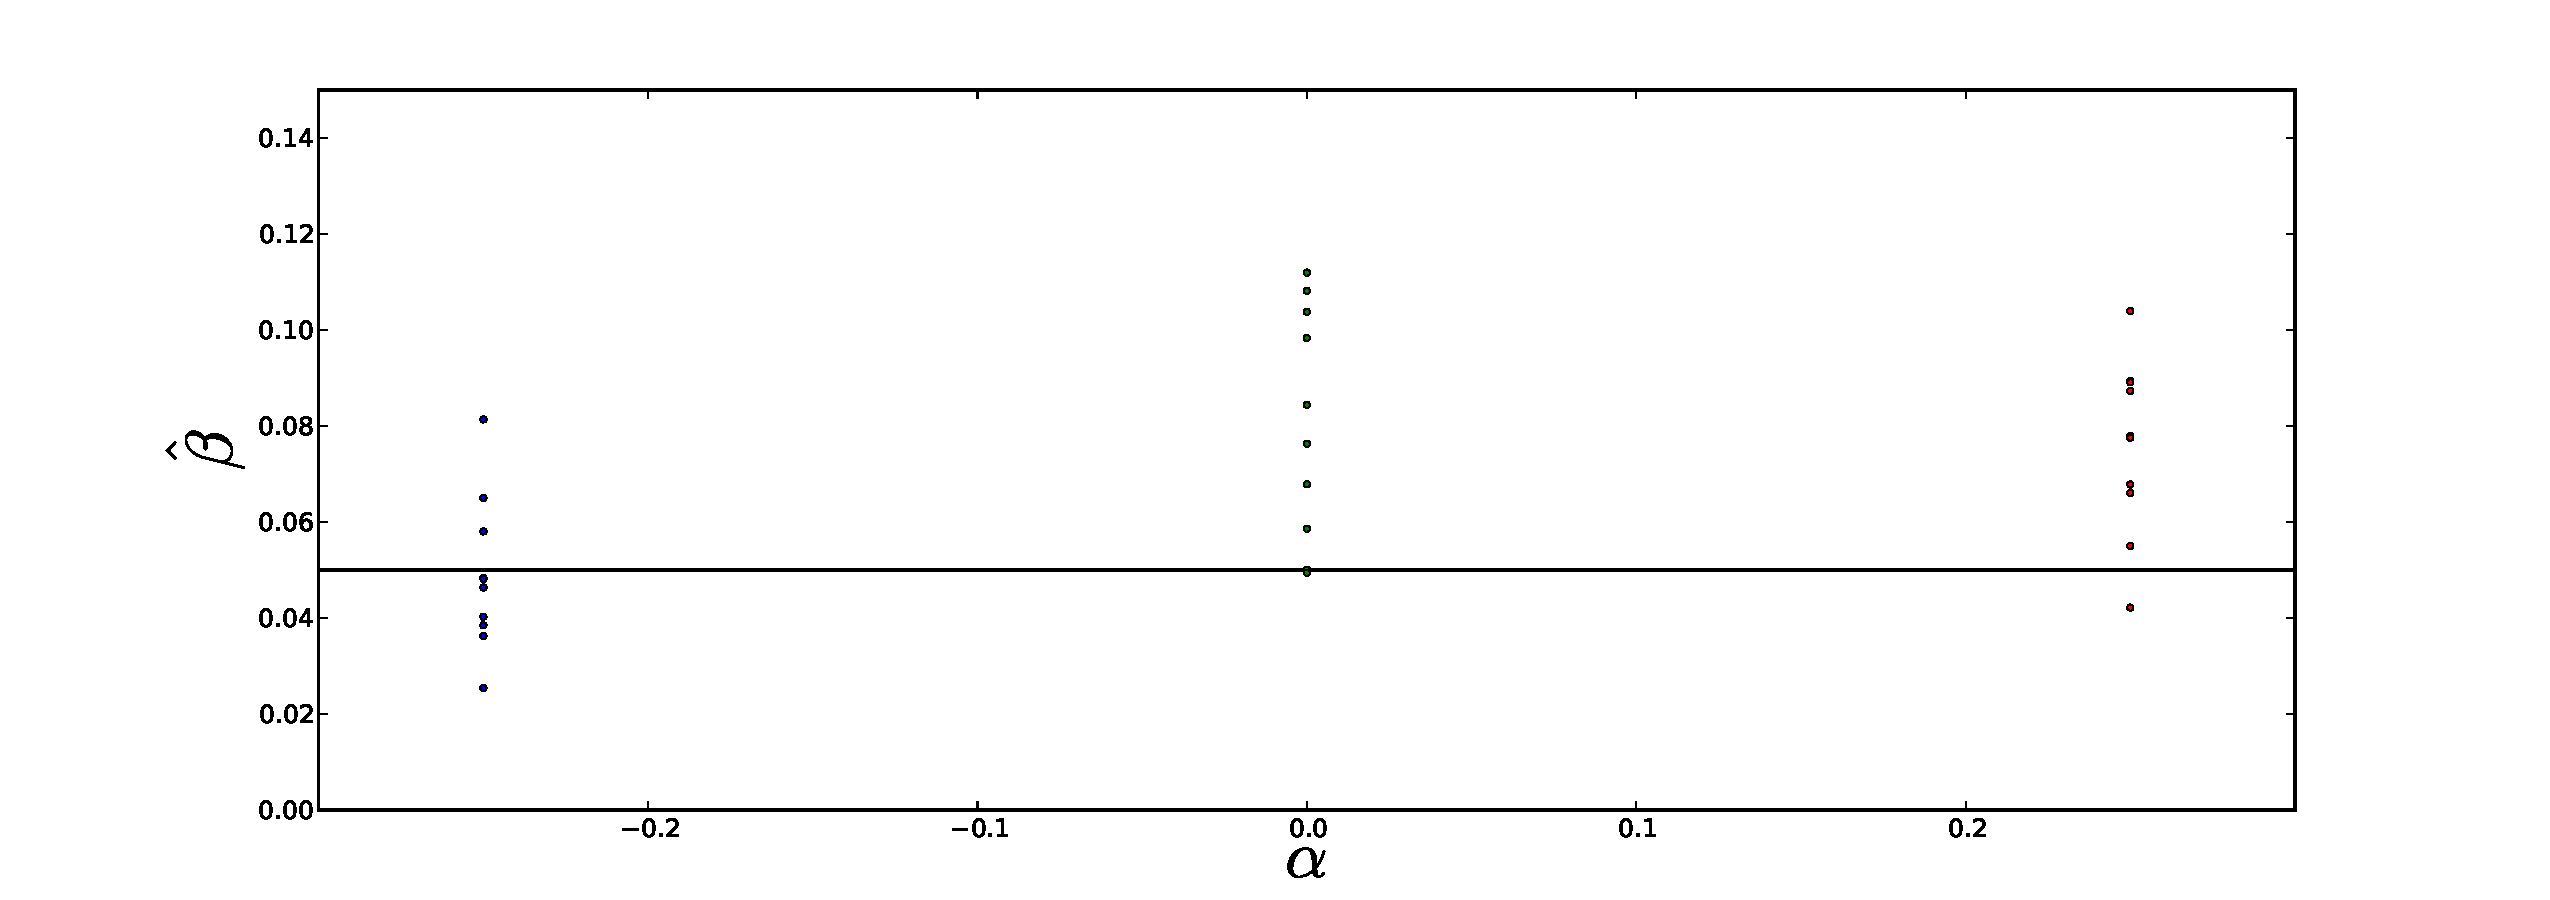
\includegraphics[width=1\textwidth]{Figs/MIML/perturbed_estimates.pdf}
\caption[]{The estimates for $\b$ given the three perturbed
trajectories (one is actually un-perturbed ($\a=.0$)). The solid black line
indicates the true value of $\b$}
\label{fig:perturbed_estimates}
\end{center}
\end{figure}

\subsection{Bang-Bang?}
We expect that it is actually best to apply maximum inhibition or maximum
excitation. That is we expect that $I(\a_2) > I(\a_1)$ for $|\a_2| > |\a_1|$. We
verify this in \cref{tab:MI_bang_bang_alphas}, where we see the general tendency
that bigger is more informative than smaller and negative is more informative
than positive.
\begin{table}
\begin{centering}
\begin{tabular}{cc}
$\a$& $I(\a)$ \\
-2&  2.31 \\
-1.00 & 1.714 \\
-0.50 & 1.182 \\
0.50 & 0.885 \\
1.00 & 1.563 \\
2 &  2.20 \\
\end{tabular}
\caption{values of MI}
\label{tab:MI_bang_bang_alphas}
\end{centering}
\end{table}
\Cref{tab:MI_bang_bang_alphas} and our intuition suggest then that the choice
for which is always between the two extremes st.\ $\a_{\textrm{most
informative}} \in \{\amin, \amax\}$.

Now we wonder what happens to the calculated value of $I$ as we move $\Delta_f$,
see \cref{fig:MI_delta_f_variation}. Now this is interesting. As $\Delta_f$
increases, we have a raise in the mutual information. Intuitively this is
obvious, since bigger $\Delta_f$ means more data. However, recall that we are
only considering the information contained in the final value (at $t=\Delta_f$).
That is also why $I$ levels off eventually, if we were considering the full path
and not just the final value, then it should continue increasing monotonically,
although perhaps with a decreasing slope. However! It is also clear that while
in the current context and for the current example at this time, inhibition is
best $I(-) > I(+)$. At some point in the future excitation will be better! That
is as the $X$ variable settles into its new, lower, equilibrium, $I(+) > I(-)$.

The question becomes how to formulate this problem as to decide on when to
switch. 

%\usepackage{graphics} is needed for \includegraphics
\begin{figure}[htp]
\begin{center}
  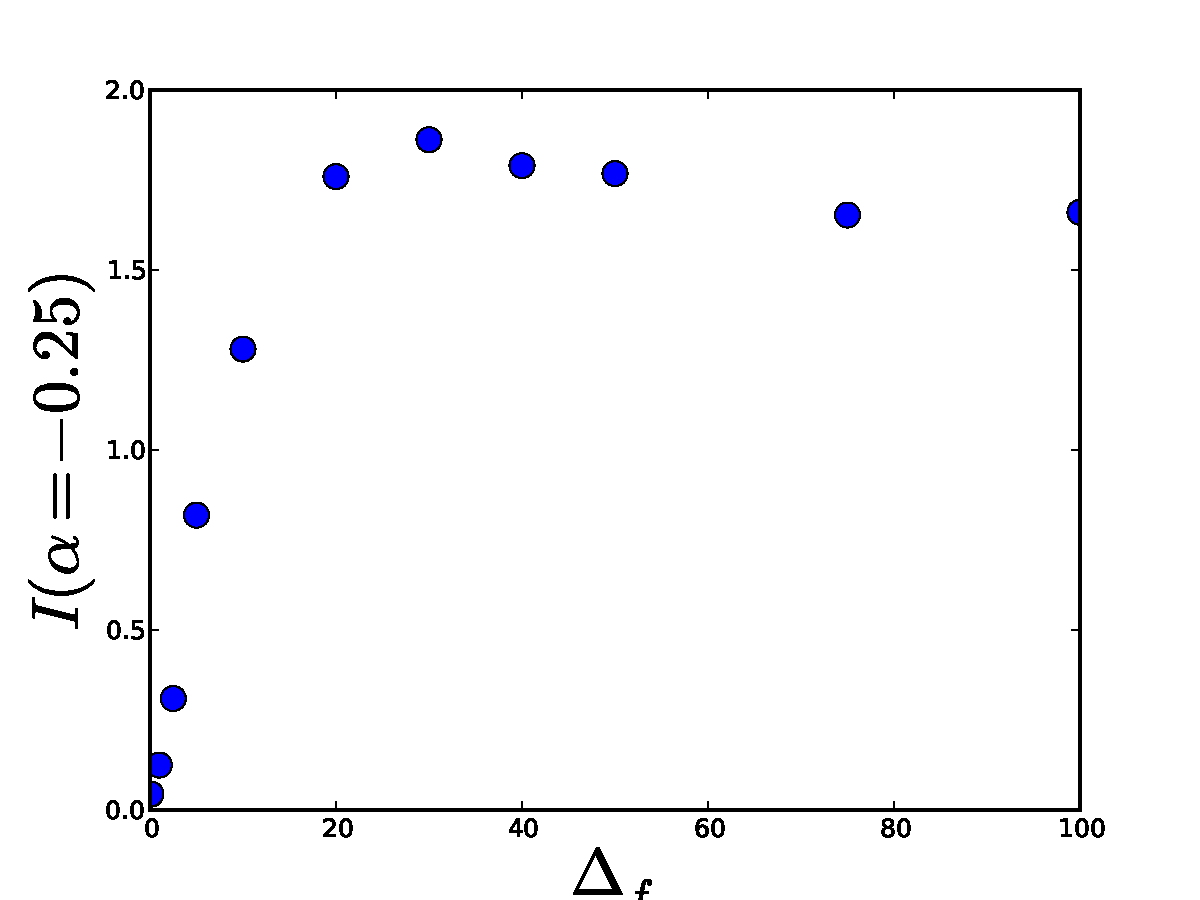
\includegraphics[width=1\textwidth]{Figs/MI/forward_deltas_vs_MIs.pdf}
\caption{values of MI while varying $\Delta_f$. Note that the right-most value
is a little iffy, as the integration routines warn about possible problems with
the variuos integrals}
	\label{fig:MI_delta_f_variation}
\end{center}
\end{figure}
Let me explain why, potentially, this is an interesting problem, what is a
possible solution and why that solution is possibly very difficult to enact:

\subsubsection{Optimal Switching for Optimal Design}
Let us recap where (we think) we are:
There is an observed OU process $X_t$. We estimate it on the fly and have
estimates for $\b, \m, \s$ or more precisely we have a distribution for $\b$ and
a one-to-one relation between $\b$ and $\m,\s$. 

We have a control of $\a$ with which we can stimulate $X$. We want to use $\a$
to improve the observations of $\b, \m, \s$. We use the Mutual Information
criterion, $I(\a)$ to select $\a$. From the structure of the OU process, it is
conjectured and empirically observed that the bigger in magnitude $\a$ the more
informative it will be. Thus, in the absence of an energy cost, we are left only
to select between the two extreme values of $\a$, $[\amin, \amax]$, which
we can assume to be just $[\pm \amax]$ for some $\amax>0$. Thus at any time, $t$,
we can calculate $I(\amin), I(\amax)$ and choose the $\a$ associated with the larger $I$.

However, in a sense this is greedy and thus not necessarily optimal.

Here is a simple way to think about it:

Imagine that $\amin, \amax$ correspond to two equilibria
$\xmin, \xmax$. Our intuition is that there is a mid-point $\xmid$ between
$\xmin, \xmax$ st. if $X_t < \xmid$, we should apply $\amax$ and conversely. 
It is now clear that this can easily result in chattering - being below $\xmid$
we stimulate which sends us above $\xmid$ and then we inhibit, since above
$\xmid$ it is most informative to inhibit and so on. 

When you add the noise, it is hard to see if that is even a better idea than
doing nothing. 

Of course, things are not so simple as the distribution on the parameters,
$\rho$ may make $\xmid$ itself move as $\rho$  shifts and shrinks, but let's
ignore that for now. 

At this point it becomes clear that we need a way to choose the switching time
to switch between  $\amax, \amin$ using something more sophisticated than just
the instantaneous value of $I(\a)$. This is related to the problem of
how to choose the observation time $\Delta_f$ in the formulation of $I(\a)$. 

Basically we need to select what we are going to do now in part based on what we
can do later. And that is Dynamic Optimization!

The main difference here from standard Dynamic Optimization is
that our state is not so much the value of $X_t$ but the value of $\hat \b_t,
\hat \m_t, \hat \s_t$, the estimates at time $t$. Once we realize this, we also
realize our main challenge - the updates for $\b, \m, \s$ using the ML
formulas are non-Markovian! That is we look back on all the old
data when taking the new data into account to form $\hat \b_t, \hat \m_t, \hat
\s_t$. 

So we need to do one of two things
\begin{enumerate} 
  \item come up with a heuristic way of choosing $\Delta_f$ before which to
  consider switching (if $\Delta_f$ is large enough, we will always switch (I
  think))
  \item Come up with an incremental form for updating $\b$
\end{enumerate}

Since route 2 leads to Dynamic Programing type equations, we follow it. 

\subsection{Framing the Problem as a Dynamic Program}
FROM HERE ON IT IS ALL SPECULATIVE AND MIGHT AS WELL OMIT READING

Let us assume that we have figured out how to update $\b$, equivalently
$\rho(\b)$ truly based on Bayesian updates, i.e. Markov-like. A very crude
method to this end is to take the posterior and simply project it onto a
Gaussian\ldots

Here comes the second challenge - roughly speaking we have an infinite
dimensional state space - the belief distribution of $\b$. Now, as soon as we
parametrize the belief distribution to a normal with mean variance $\bar \b,
\s_b^2$ then we are back to finite dimensions and we are good to go. 

We will consider framing the problem as a discounted infinite-horizon dynamic
program:
\begin{equation}
v(\rho_t(\b), X_t) = \max_{\a_k} \sum_{k \geq 0} \g^k  I(\a_k, \Delta_k;
X_k, \rho_k(\b))
\end{equation}
where $\g \in (0,1)$ is an arbitrary discount factor and $\Delta_k = t_{k+1} -
t_k$ is the forward increment which is assumed fixed. A simplification thus is
that we assume the observation times are a priori known and fixed.

So as long as we figure a smart way to update the parameter belief
distribution(s) online, we can then try to solve the Bellman equation for
infinite horizon, discrete-step problems:
\begin{equation}
v(x_0, \rho_0) = \max_{\a \in \{\amin, \amax\}}  \bigg[ I(\a, \Delta_0; x_0,
\rho_0(\b)) + \g \Exp_\a [ v(x_1, \rho_1)] \bigg] 
\label{eq:MI_bellman_infinite_horizon}
\end{equation}
and then choose the optimal stimulus simply as:
$$
\a = \argmax_\a \bigg[ I(\a,  \Delta_0, x_0, \rho_0(\b)) +
		 \g \Exp_\a [ v(x_1, \rho_1)] \bigg]
$$
On one hand this looks deceptively simple. On the other it is strictly 
more complicated than the greedy approach where $\a$ is selected 
based on:
$$
\a_{\textrm{greedy}} = \argmax_\a \bigg[ I(\a,  \Delta_0; x_0, \rho_0(\b))\bigg]
$$ 
If the calculation of the mutual information $I$ is expensive (as so far it has
been), we can rule out small $\Delta_f$ i.e.\ small $\Delta_0$, at least in the calculation of the
switch times. We can still observe at a higher frequency.

A few more words on the value function, $v$ and its arguments $x_0, \rho$. If we
take the Gaussian approximation for $\rho(\b) \sim N(\bar \beta, \sigma_\b)$
then $v(x_0, \rho) = v(x_0, \bar \beta, \sigma_\b)$, which is just a
3-dimensional function. If we want to have a full prior, $\rho(\m, \b, \s)$ then
we will have a 1+3+6-dimensional function. Already at $d=3$, but certainly at
$d=10$ we will need to apply some kind of function approximation to $v$. 
$$v(\ldots) = \sum_j r_j \phi_j (\ldots)$$
where $\phi_j$ are appropriately chosen basis functions. 

Let us dissect  a little bit \cref{eq:MI_bellman_infinite_horizon}. In
particular what is $\Exp_\a [ v(x_1, \rho_1)]$? Well the expectation is taken
with respect to what is random, i.e.\ the next realization of $X$, that is the
value of $X_{t+\Delta_0}$. But $X_{t+\Delta_0}$ must further be conditioned on
the current value of the belief distribution.  
So
$$ \Exp_\a [ v(x_1, \rho_1)] =
\int_{\{X, \th\}} v(x, \rho_1(|x)) L(x|\th) \rho_0(\th)
\intd{\th}
\intd{x}
$$
We write $\rho_1(|x))$ as a reminder that the posterior depends on the
realized value $x$. Basically, for every possible $\th, x$ in the joint
forward density, we need to consider what will be the updated $\rho_1$. And thus
we need an efficient way to update $\rho_1$. 

We now explore in turn the two main challenges:

\begin{enumerate}
  \item How to update the prior $\ra$ posterior efficiently
  \item How to solve the bellman equation, \cref{eq:MI_bellman_infinite_horizon}
\end{enumerate}

\subsubsection{Updating the Prior on the fly}
Recall that the great disadvantage of the ML formulas for $\b, \m, \s$ is that
they are not recursive. Moreover the bootstrap approach to form priors is
even more non-recursive:-! This robs us of a Markovian structure, and in turn we
cannot use Dynamic PRograming techniques / the bellman equation.

We need to be more shrewd. 

Note that the parameter belief distributions is only used to guide the online
OptDesign process, i.e.\ the on-the-fly seclection of $\a$. There is nothing
stopping the analyst in using the ML formulas once all the data has been
collected.

Thus, we can hope that we can use a less efficient estimator than ML as long as
it is roughly correct. In particular having the wrong value of $\s_\b$ shouldn't
be a big deal\ldots In fact, from messing around with the routines, it seems the
only thing that is really of any importance is that $\s_\b$ is not zero. If it
were zero then $I(\a)=0\, \forall \a$, which is reasonable since $X$ carries no
additional information on the already fully specified parameter set $\th$. Other
than that, wildy different values for $\hat \b, \s_\b$ seem to give the same
ordering between $I(\amin), I(\amax)$\ldots This is a little strange, since it
looks like the prior doesn't really matter\ldots but let us move on for now.

Ok, how do we efficiently update the belief distributions given a new
observations, and approximately if necessary. 

Let us make it hard for ourselves at first. Assume a joint prior $\rho(\m,
\b,\s)$.

Then the posterior is
$$
p(\m,\b,\s | x) &= \frac{L(x|\th) \cdot \rho(\th) }{\int_\Theta L(x|\th)
\rho(\th) \intd{\th}} $$
where the likelihood is given by 
$$
L(x|\th) = \frac{\b}{\s \sqrt{(1 -  e^{-2\b \Delta_0}})}\cdot 
\exp\left(\frac{\left( x - (\frac \a\b + \mu)  - (x_0 - \frac \a\b - \mu)
\cdot e^{-\b \Delta_0} \right)^2 \cdot \b}
			{ \s^2  (1-e^{-2\b\Delta_0})} \right)$$

So what is a good way to update $\rho\ldots$. Well, in a sense what we have here
is a (simple) filtering problem. $\b,\m,\s$ can be thought as the unknown
(hidden) process which is actually static, while $X$ is the observation process.
Assuming that we cannot close-form the updates for the posterior, which is the
same as stating that we cannot find in analytical form a conjugate
prior, we need to open the toolbox of filtering theory, such as one of 
\begin{enumerate}
  \item Extended Kalman Filters
  \item Particle Filters
  \item Sigma-Point (Unscented Kalman) Filters
  \item \ldots
\end{enumerate}

% \subsubsection{An SDE for updating the paramters}
% Here is a cute alternative: given a cts observation of $x$ the likelihood is
% known. And the log-likelihood as well: 
% 
% If 
% $$
% dX = f(X; \th) dt + \s dW 
% $$
% assume a simple 1-D process with known volatility $\s$ and unknown params in the
% drift vector. Then the log-likelihood of a trajectory $X_0^T$ is
% $$
% l(X; \th) = \int_0^T -\frac {f^2}{2\s^2} dt + \frac f\s dW  
% $$
% 
% Then suppose that we have a guess for the parameter vector $\th_m$, then we can
% use the gradient of $\l$ with respect to $\th$ as the update:
% $$
% d\th_m = s \grad_\th (dl(\th_m))
% $$
% where $s$ is a step size (akin to a Newton-type method). We write $\th_m$ to
% differentiate it from $\th$. $\th_m$ is a guess or an estimate for the parameter
% value, while $\th$ is the 'true' parameter under which $X$ evolves. 
% 
% What is $dl(X, \th)?$, well, we can read that directly. 
% $$
% dl(X,\th) = -\frac {f^2}{2\s^2} dt + \frac f\s dW
% $$
% and thus
% $$
% d\th_m =  s \left[ -\frac {f(X, \th_m) \cdot \grad_\th f(X, \th_m)}{\s^2} dt +
% \frac {\grad_\th f(X, \th_m)}\s dW \right]
% $$
% 
% Let us recap. $X$ is evolving under its true parameter $\th$, while $\th_m$ is
% evolving under the gradient flow $\grad_l$, more importantly, the $dW$ in both
% is the same\ldots. Ah wait, in practice we won't know the value of $dW$\ldots
% just $dX$. Right, $dW = (dX - fdt) / s$. So we do know $dW$.
% 
% Anyway\ldots this doesn't work actually. 





\subsubsection{The Value function}
Here comes the tricky part. Any of the above will allow us to form an
approximate posterior, $p$. But will any of them be usable in the DP formulation
above? The simplest case is if $v$ only depends on 2-nd order
statistics of $p$. Then we can just ask  the approximate posterior for its 2-nd order stats
and then plug them into $v$

Thus all we need to do is calculate the moments:
$$\bar \th (x) = \int_\Th \th \cdot p(\th|x) \intd{\th} 
= \int_\Th \th  \cdot \cdo \frac{L(x|\th) \cdot \rho(\th) }{\int_\Theta L(x|\th)
\rho(\th) \intd{\th}} \intd{\th}  $$
and
$$\Xi_\th(x) = \int_\Th  (\th - \bar \th) : (\th - \bar \th)\cdot p(\th|x)
\intd{\th} 
= \int_\Th  (\th - \bar \th) : (\th - \bar \th)\cdot \cdo \frac{L(x|\th) \cdot
\rho(\th) }{\int_\Theta L(x|\th) \rho(\th) \intd{\th}} \intd{\th} 
$$
where we use $:$ to write the outer product to form the variance (we only need
to calculate the upper triangle of the matrix).

and then have $v(x, \rho) = v(x, \bar \th ,\Xi_\th)$. This makes $v$ a function
of 1+3+6 parameters, if we have 3 unknown params, $\m,\b,\s$

Let's take a step back - to calculate the value function, we now need to
calculate:
$$ \Exp_\a [ v(x_1, \rho_1)] =
\int_{\{X, \th\}} v(x, \rho_1(\th|x)) L(x|\th, \a) \rho_0(\th)
\intd{\th}
\intd{x}
$$
and then for each value of $x$ inside the integral we need to further calculate
what the moments of the posterior would be using the moment updating equations
above (or others). That is just to evaluate the expectation of the value
function.

In the best case, when we need to choose over only two values of $\a$, we will
have to evaluate $I, v$ twice, once for each alternative $\a$. 

What we need to hope for is that a rough approximation for $v$ will be good
enough\ldots

\subsubsection{Cts-time observations}
Sometimes things are easier if they are stated in continuous time. Let $f(x_t,t|
x_0, 0 ; \th)$ be the forward density of $x$ given $\th$. $f$ is a soln to the
Forward Kolmogorov/ Fokker-Planck equation. Then the mutual information is the
limit of:
\begin{align*}
I(X,\th) =& \int_\th \int_{X_{t_1}}\cdots\int_{X_{t_n}}
 \log
 \left(\frac{\prod_n (f(X_{t_{n+1}},t_{n+1}|X_{t_{n }},t_{n} ;\th)}
 {\int_\th \prod_n (f(X_{t_{n+1}},t_{n+1}|X_{t_{n }},t_{n} ;\th)
 \rho(\th) \intd{\th} }\right) 
 \\&\cdot 
 \prod_n (f(X_{t_{n+1}},t_{n+1}|X_{t_{n }},t_{n} ;\th) 
 \cdot \rho(\th) \intd{x_1}\cdots\intd{x_n}\intd{\th} 
 \end{align*}
as $X_{t_n}$ refines to the full cts-time trajectory $X_t$. It is clearly unfeasible to evaluate $I$ as we must do an infinite number of joined integrals.
The only approach is to do a Monte Carlo integration using $X_t$ trajectory
samples.

However one may try to pose the problem in the more simplistic average of each
time:
$$
\tilde I(X,\th) = \int_\th \int_0^T\int_X
 \log\left(\frac{f(x,t|\th )}{\int_\th f(x,t|\th) \rho(\th)}\right) 
 f(x,t|\th) \cdot \rho(\th) \intd{x}\intd{t}\intd{\th}
$$
Once again, $\tilde I$ is not the mutual information, $I$ is. But the equation
to maximize $\tilde I$ looks like a dynamic programing problem. It can also be
written as:
$$
\tilde I(X,\th) = \Exp_{\th} \Exp_{X_t}
\left[ \int_0^T \log\left(\frac{f(x,t|\th )}
{\int_\th f(x,t|\th) \rho(\th)}\right) \intd{t} \right]
$$
which is the form necessary to apply the dynamic programing equations, except
that we have an extra expectaton (wrt. to the parameter prior):


\subsubsection{the value function in cts. time}
NOTE: THIS IS A MESS

Instead we might find that working in cts. time makes things easier for us. 
\begin{equation}
v(\rho(\th), x) =
\max_{\a_k} \Exp\left[ \int_{t \geq 0} e^{-\g t}  i(\a_k, dt; X_t, \rho_t(\th))
\intd{t}\right]
\label{eq:mutual_info_objective_cts_time}
\end{equation}
where $i$ is the infinitesimal mutual information for a small interval $dt$

$$
i(\a_k, dt; X_t, \rho_t(\th) = 
$$
Now we know that the continuous time-likelihood $L$ in general for a stochastic
process
$$
dX = f dt + \s dW
$$
over the interval $[0,t]$ is
$$
L(X) = \int_0^t \frac {-1}{2} \frac{f^2}{s^2} dt + \frac{f}{s}dW
$$
where the $W$ in the integral corresponds to the one that generated the data
$X_t$.

Now we are trying to maximize the running reward
$$
\Exp [ \int_0^\infty e^{-rt} i(X_t, \rho_t(\th); \a)\intd{t}]
$$
where $i$ is the infinitesimal mutual information between $X_t+dX$ and the
posterior $p(\th) \sim \rho_t(\th) + d\rho$.
The value function is written as: 
$$
v(x_0, \rho_0(\th)) = \sup_{\a} \Exp[\int_0^\infty e^{-rt} i(X_t, \rho_t(\th);
\a)\intd{t}
$$
Now for $\th$ fixed. This leads to the Bellman equation:
$$
0 = -r v(x, \rho) +
 \sup_\a[ i(x, \rho; \a) +
 \frac{\Exp[v(x + dx, \rho + d\rho)]] - v(x,\rho)}{dt} \quad \forall
 x_0, \rho_0 $$ 
The interesting term in this expression is, of course, 
$$
\frac{\Exp[v(x + dx, \rho + d\rho)]] - v(x,\rho)}{dt}
$$
If $v$ were a function of $x$ only then this would be just
$$
\frac{\Exp[v(x + dx)] - v(x)}{dt} = \int_\th \Lstar_{\th, \a} [v] \cdot
\rho(\th) \intd{\th} $$
where $\Lstar$ is the generator for $X_t$'s diffusion given fixed, $\th,\a$
i.e.\
$$
\Lstar [\cdot] = f(x; \th, \a) \cdot \di_x[\cdot] + \frac{\s^T \s }{2}: \di^2_x
[\cdot] $$
HOWEVER!
if $v$ is a function of both the observation and the current belief
distribution $X_t, \rho_t$, things become more complicated since the posterior
depends on $X$
i.e. 
$$
v(x+dx, \rho+d\rho) = v(x+dx, \rho(x+dx))
$$
This means that when we do things like take $x$-differentials, $\di_x v$, we
must take total differentials
$$
\di_x v =  \di_1 v(x, \rho(x)) + \di_2v(x, \rho(x)) \cdot \di_x (\rho(x))
$$
where we write $\di_1,\di_2$ to indicate we are differentiating with respect to
the first or second argument of $v$
Now what is $\di_\rho$? Well, for fixed $\th$, $\rho(\th|x)$ is just a number.
it is the probability or probability density of $\th$ given $x$. So for fixed
$\th$ $\di_\rho$ is a single variable derivative.

So we are left to wonder what is the shape of the derivative of the posterior
wrt $x$ evaluated at $x_0$ (the last observation).

This is not obvious. Let's start from the posterior-prior definition (i.e.\
Bayes rule):
$$
p(x) = \frac{L(x|\th) \rho(\th)}{ \int_\th L(x|\th') \rho(\th') \intd{\th'}} 
$$
For small $dt$, the likelihood $L(x)$ is a highly peaked normal, centred at
$x_0$ with variance $dt$. 
$$
p(x) = 
\frac{\exp(-\frac{(x- (x_0 + f(x_0, \th) dt))^2}{2\s^2 dt}\cdot
\rho(\th))}
{\int_\th \exp(-\frac{(x- (x_0 + f(x_0, \th) dt))^2}{2\s^2 dt}\cdot
\rho(\th) \intd{\th} } $$
Now $\di_x p = \di_x \log(p) \cdot p$, so we will try to calculate the
derivative of the log instead
$$
\log(p(x)) = -\frac{(x- (x_0 + f(x_0, \th) dt))^2}{2\s^2 dt} +
\log(\rho) -
\log({\int_\th \exp(-\frac{(x- (x_0 + f(x_0, \th) dt))^2}{2\s^2 dt}\cdot
\rho(\th) \intd{\th} } )
$$
Taking its derivative
\begin{align*}
\di_x \log(p) =& -\frac{(x- (x_0 + f(x_0, \th) dt))}{\s^2 dt}
\\ 
&- \frac{\int_\th -\frac{(x- (x_0 + f(x_0, \th) dt))}{\s^2 dt} \cdot \exp(-\frac{(x- (x_0 + f(x_0, \th)
dt))^2}{2\s^2 dt}\cdot \rho(\th) \intd{\th} }
{\int_\th \exp(-\frac{(x- (x_0 + f(x_0, \th) dt))^2}{2\s^2 dt}\cdot
\rho(\th) \intd{\th} }
\end{align*}



The crudest thing to say is that $ \di_x (\rho(x))= 0$! B/c if it is not, the
complications become untenable. 

Then the dynamic programing equation reduces to: 
\begin{equation}
0 = \sup_\a \left\{ i(\a, x, \rho) +
\int_\th \L_\th^*[v(x, \rho(\th))]\cdot \rho(\th)\intd{\th} - \g v(x,
\rho(\th))\right\}
\label{eq:HJB_mutual_info_inf_horizon}
\end{equation}
for all possible state-points $x$, and priors $\rho$.
As this is an infinite-dimensional state-space problem, we need to have a way to
truncate $\rho$ to a finite dimension.

How we solve \cref{eq:HJB_mutual_info_inf_horizon} is discussed next.


\subsubsection{Value function approximation}
Value function approximation refers to approximting $v$ with a pre-determined
basis:
$$
v(x,\rho) = \sum_k r_k \phi_k (x, \rho)
$$
The art is choosing the functions $\phi_k$ so as to fit the problem. A good
choice of $\phi$ will mould to the actual (but unknown) shape of $v$.

I can't right now come up with obvious examples of $\phi$ that will be
appropriate. A common generic choice is tensor-products of Chebyshev polynoms
up to order 3. 


\clearpage
\section{Gauss-Hermite Integration}
\label{sec:gauss_hermite_integration}
NOTE: THIS DOES NOT WORK FOR NOW, SO THIS SECTION IS OPTIONAL READING:

Gauss-Hermite integration is a well-known technique for Gaussian
quadrature on the Real axis with a Gaussian weight: i.e. how to integrate:
\begin{equation}
I(f) = \int_\R f(x) e^{-x^2} \intd{x}
\label{eq:standard_hermite_integral}
\end{equation} 
The general theory is in sec 4.5 of \cite{Press1992}, here we just cite the
results:
\begin{equation}
I(f) =  \sum_j^d w_j f(x_j)
\end{equation}
where the weights and nodes $w_j, x_j$ are related to the roots of the Hermite
polynomials of order $d$. (We use a function in numpy, hermite.hermgauss, to
obtain them for a given $d$).

This suffices to integrate against an arbitrary Gaussian weight. How?
\begin{align*}
I(f) =&
\frac{1}{\s_y \sqrt{2 \pi}} \int_\R f(y) e^{-\frac{(y-\bar{y})^2}{2\s_y^2} }
\intd{y} 
\\ 
=&
 \frac{1}{\sqrt{\pi}} \int_\R f( \sqrt 2 \sigma_y x + \bar y)e^{-x^2}
\intd{x}
\\ 
=& \frac {1}{\sqrt{\pi}} \sum_j w_j f(\sqrt 2 \sigma_y x_j + \bar y )
\end{align*}

To relate this explicitly to our case above, integrals of against the $\b$ prior
can be calculated as:
$$
I(f) = \int_\R f(\b) \rho(\b) \intd{\b} = \frac {1}{\sqrt{\pi}} \sum_j w_j
f(\sqrt 2 \sigma_\b x_j + \bar \b ) $$
I.e. we just shift and scale the generic variable $x \ra \sqrt 2 \sigma_\b x +
\bar \b$.

Our problem above consists of a double integration, where the $x$ variable is
normal conditional on $\b$, but the two are certainly not jointly  normal! So we
will proceed as follows:

We lay out a gauss-hermite grid of nodes for the $\b$ variable and then for each
beta node, we will lay out a gauss-hermite grid for $x$. 

At this point it again worth pointing out that a pure normal distribution for
$\b$ is a bad idea! And cutting off the nodes for $\b<0$, works (roughly), but
spoils the spectral convergence of the quad-rule. For now we continue with
this bad prior, just so we can compare with our previous results. 

We visualize the node-spread in \cref{fig:hermite_nodes}. It looks like we only
need about 9 nodes in the $\b$ direction. However when we attempt to duplicate
the marginal figures from \cref{fig:marginal_px}, we run into complications. See
\cref{fig:marginal_px_gauss_hermite}. In particular even at high nodes, we run
into this blip for the forward density of $X$ for $\a = =.25$. In general this
is probably not there. We think it appears because the likelihood of $X$ which
is being integrated against the prior of $\b$ is not sufficiently smooth. IN
particular, Gauss-type quadrature works best for functions that are low-order
polynomials or at more generally that are analytic with a power-series
representation that drops off sufficiently fast. Now, for fixed forward $X$ the
likelihood has a term of the form $\a / \b$. This may be the cause of the blip
on the right. (Note that there is no blip for
$\a=0$ in \cref{fig:marginal_px_gauss_hermite}). Still, the fact that the overall shape is
maintained, leads us to move on. 
\begin{figure}[h]
\begin{center}
\subfloat[node distribution]
{
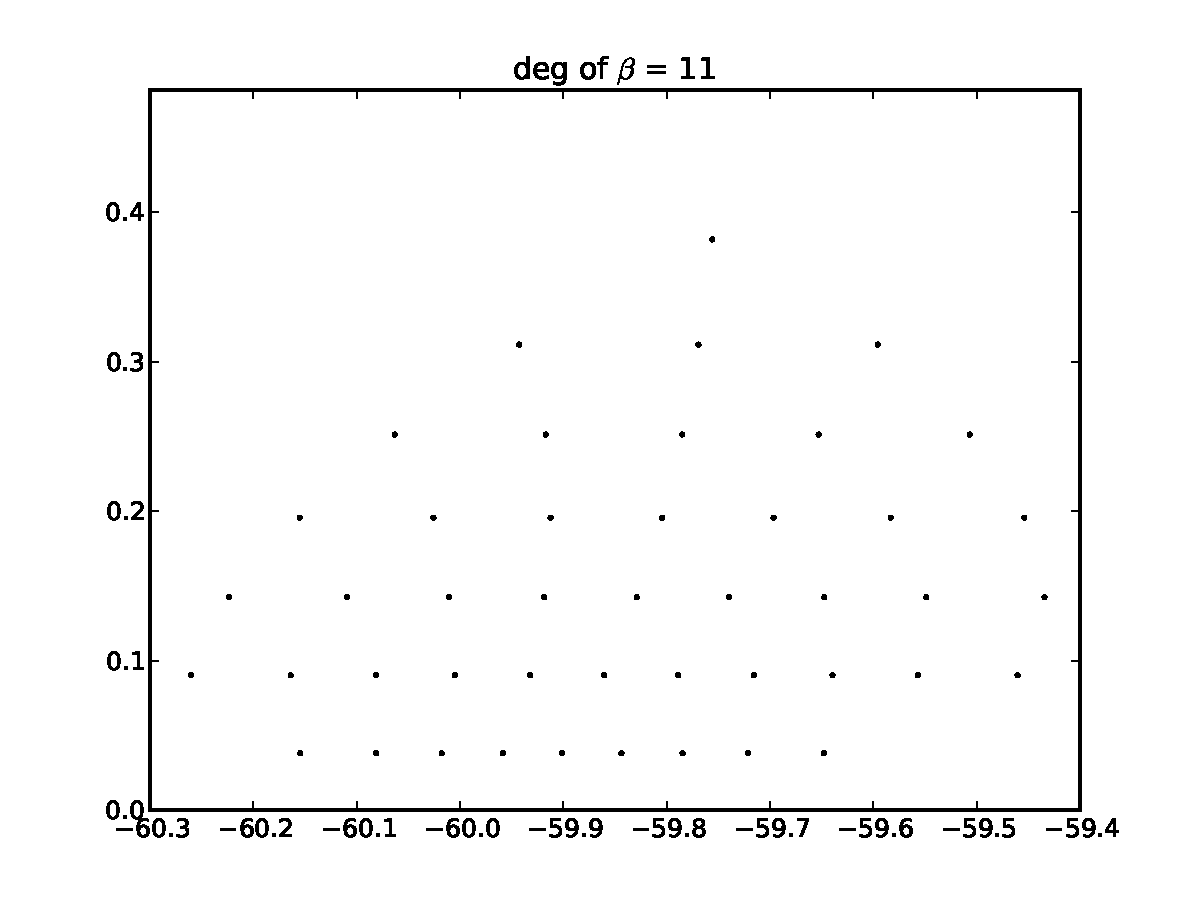
\includegraphics[width=0.48\textwidth]
{Figs/HermiteBox/nodes_spread.pdf}
}
\subfloat[node distribution]
{
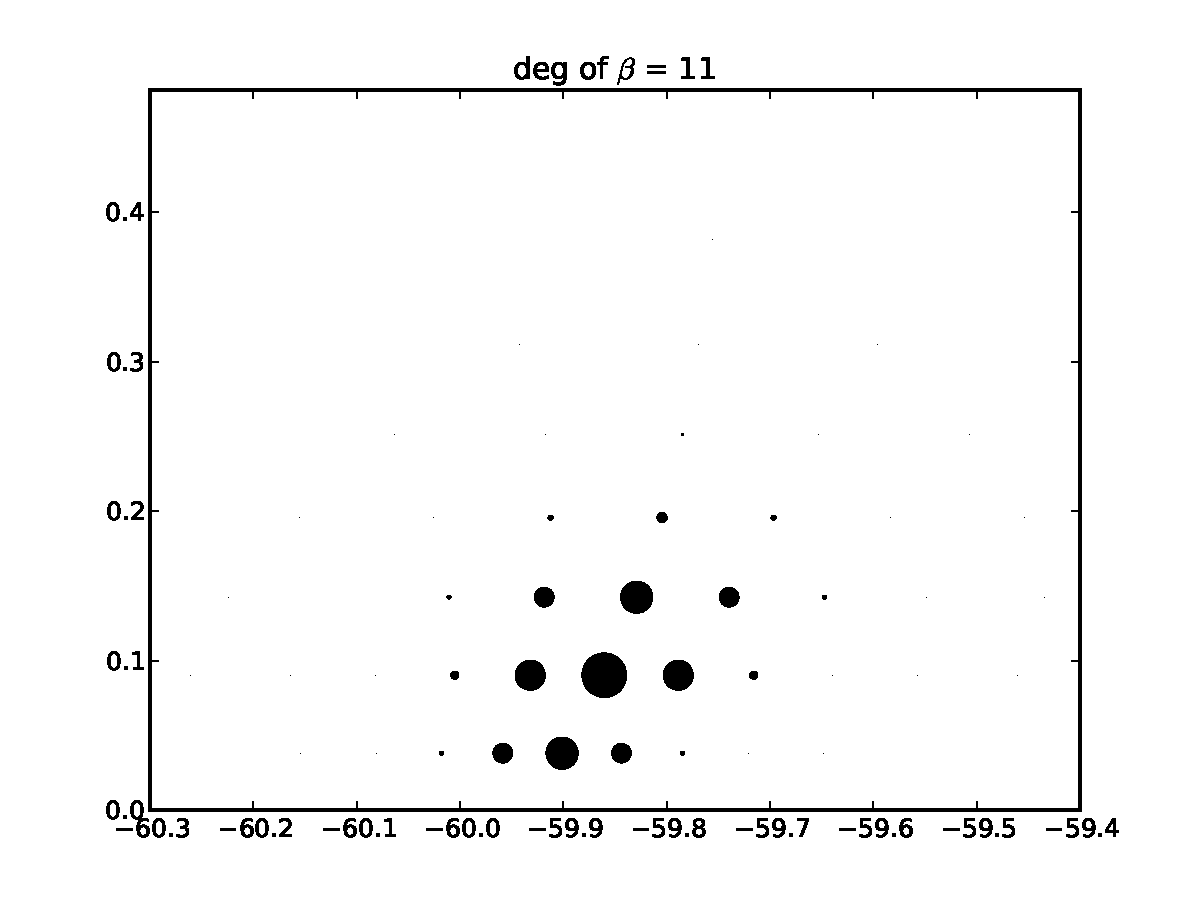
\includegraphics[width=0.48\textwidth]
{Figs/HermiteBox/weighted_nodes_spread.pdf}
}
\caption{Spread of the nodes in the $x-\b$ domain. All the nodes
are illustrated on the left and the nodes are proportional to their weight
$w_{j,x} \cdot w_{i,\b}$. Basically more than 9 nodes in the $\b$ direction seem  
not necessary, but see \cref{fig:marginal_px_gauss_hermite}}
\label{fig:hermite_nodes}
\end{center}
\end{figure}
\begin{figure}[h]
\begin{center}
\subfloat[Coarse Nodes]
{
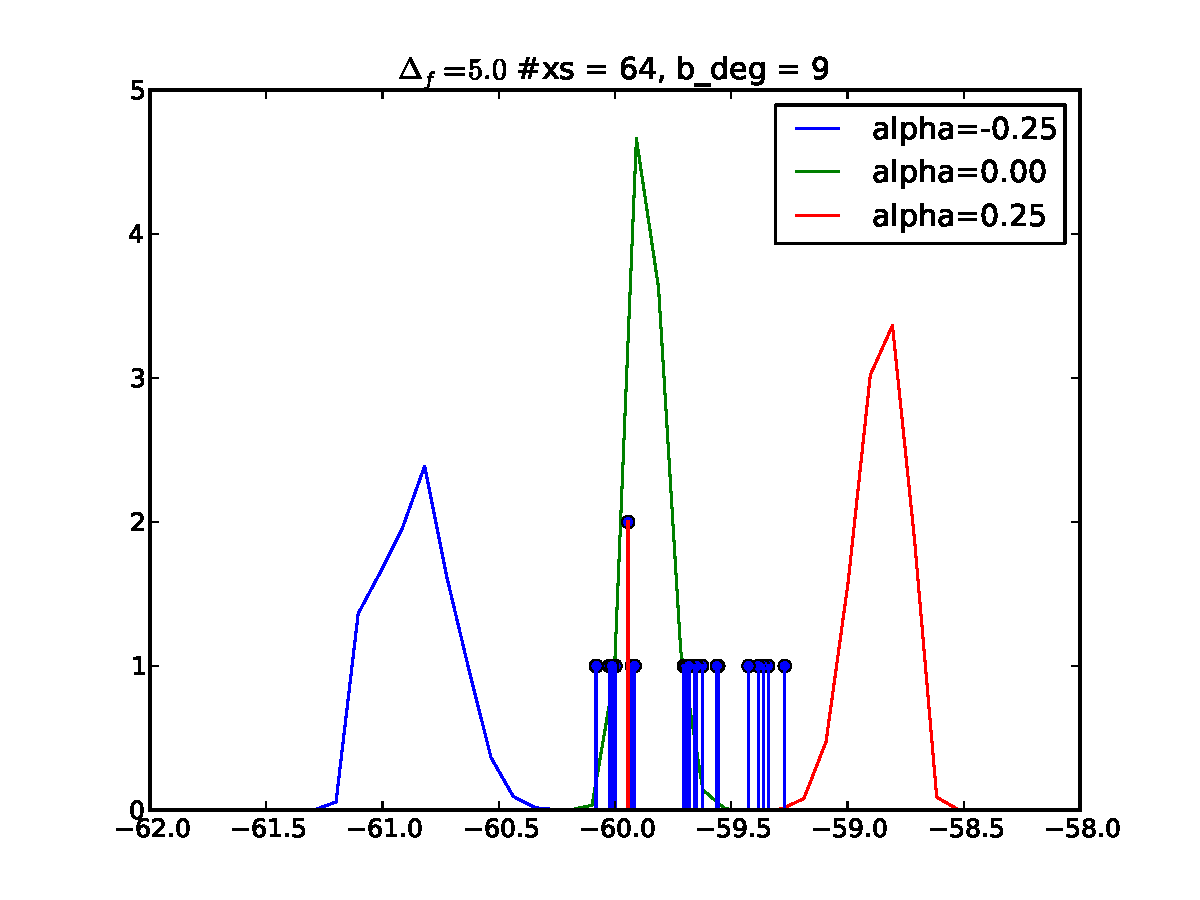
\includegraphics[width=0.48\textwidth]
{Figs/HermiteBox/x_marginal_gauss_hermite_bx=9_64.pdf}
}
\subfloat[Fine Nodes]
{
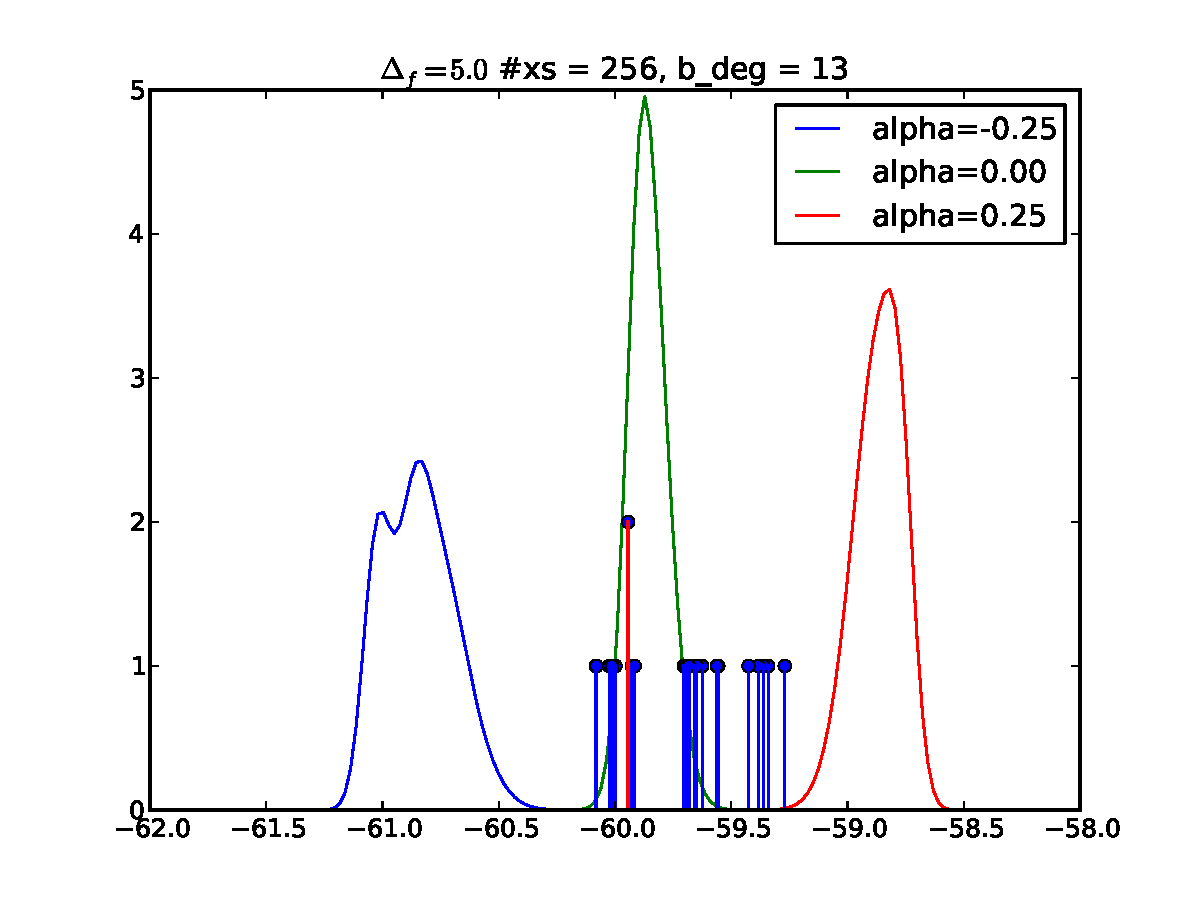
\includegraphics[width=0.48\textwidth]
{Figs/HermiteBox/x_marginal_gauss_hermite_bx=13_256.pdf}
}
\caption{The same figure as in \cref{fig:marginal_px}, but computed
with Gauss Hermite quadrature of different order}
\label{fig:marginal_px_gauss_hermite}
\end{center}
\end{figure}

We proceed as follows. For every $b_i, x_j$ node we calculate, 
$$f(x_j,\b_i) =  \log\left[\frac{L(x|\th; \a)}
										{\int_\Theta L(x|\th;\a)\cdot \rho(\th) \intd{\th}} \right]$$
										
and then we simply sum this $$I(\a) = \frac 1 \pi \sum_{i,j} w_j w_i f(x_j,
\b_i).$$ We need to be careful and keep track of the normalizing constant, which
in two dimensions is $(1/\sqrt{\pi})^2$.

The main thing to do is to try to recalculate the results in
\cref{tab:MI_3alphas_basic_quad}, but with the GH quadrature scheme. 
Hm\ldots I can't quite do it. In particular there is no convergence as we raise
the $\b$ order see \cref{tab:GH_convergence_beta}. It is a little frustrating
b/c for $d_\b = 13$ for example, the $I(-.25)$ is right. but then it goes
completely wrong. It is also frustrating, because the general ordering is
consistently maintained:
$$
I(-.25) > I(.25) > I(0)   
$$
\begin{table}
\begin{centering}
\begin{tabular}{cc}
deg($\b$) & $I(\a= [-.25, .0,.25])$ \\
7 & ['0.793', '0.132', '0.420'] \\
9 & ['0.752', '0.110', '0.380'] \\
13 & ['0.684', '0.087', '0.331'] \\
21 & ['0.824', '0.136', '0.421'] \\
43 & ['0.824', '0.135', '0.418'] \\
87 & ['0.777', '0.114', '0.384']
\end{tabular}
\caption{GH convergence of $I(\a)$ with increasing $\b$ order}
\label{tab:GH_convergence_beta}
\end{centering}
\end{table}
On the other hand, for a fixed $\b$ degree, varying the $x$ degree is almost
useless, see \cref{tab:GH_convergence_x}, convergence happens almost
instantaneously!

\begin{table}
\begin{centering}
\begin{tabular}{ccc}
deg($\b$) & deg($x$) &$I(\a= [-.25, .0,.25])$ \\
9 & 1 & ['0.7528', '0.1105', '0.3806'] \\
9 & 3 & ['0.7513', '0.1101', '0.3802'] \\
9 & 7 & ['0.7514', '0.1100', '0.3801'] \\
9 & 11 & ['0.7516', '0.1100', '0.3802'] \\
\end{tabular}
\caption{GH convergence of $I(\a)$ with increasing $x$ order, we see that using
1 for the base degree is roughly enough and 7 more than sufficient. Note that
if the deg($\b$) was any larger, than the convergence in $x$ will be even
faster (there will be no difference to 4 sig. digits between 1 and higher). }
\label{tab:GH_convergence_x}
\end{centering}
\end{table}
 
So we only need to think about what are we doing wrong in terms of $\b$. Because
for deg($\b$) fixed convergence is achieved. 

So\ldots either this just doesn't work or we have made a mistake while
GH integrating against $\b$. Let's play 'find the bug\ldots'. Well, one thing to
try is compute the normalizing constant by conventional methods ('quad' in
numpy) instead of through the GH method. Nope that has no effect (only 3rd sig.
digit effect on $I(\a)$). 
Also integrating a purely $\b$ expression like $\b$ or $(\b-\hat \b)^2$ gives
the expected results (mean, variance)\ldots

At this point I am going to suspend further efforts in this
direction \ldots although as we have seen the efficiency gains can be pretty
good (compute time on the order of .1 s to compute the $I(a)$ which once ported
to C brings us into real-time)


\clearpage
\appendix
\section{Mutual Info calculation}
Here we show why \cref{eq:mutual_info_objective} for the Mutual Information
agrees with the usual definition of the Mutual Information, which is 
$$
I = \int_\Theta \int_X p(x,\th) \cdot \log \left(
\frac{p(x,\th)}{p(x)p(\th)}\right) \intd{x} \intd{\th}$$

First of all, $p(\th) = \rho(\th)$ is just the prior of $\th$
The joint distribution $p(x,y) = L(x|\th)\rho(\th)$, while the $x$ marginal, 
$p(x) = \int_\Theta L(x|\th)\rho(\th) \intd{\th}$.
Pluging the three expressions gives:
$$
I = \int_\Theta \int_X L(x|\th)\rho(\th) \cdot 
\log \left( \frac{L(x|\th)\rho(\th) }{\int_\Theta L(x|\th)\rho(\th) \intd{\th}
\cdot \rho(\th) } \right)
\intd{x}\intd{\th}
$$
after canceling $\rho(\th)$ inside the log, we get \cref{eq:mutual_info_objective}.

\section{Relation between Mutual Information and Fisher Information}
We'd like to explore the relation between Mutual Information and the Fisher
Information in cts. time. In order to relate to the work of Hooker et al.
\cite{Lin}. 

The system is 
$$
dX_t = f(x, \th, \a) dt + \s dW
$$
st.$\s$ does not depend on $\th, \a$, but may depend on $X_t$

The corresponding cts-time log-likelihood is written as:
$$
l( \th| X_0^T ) 
= \int_0^T \frac{f^2}{2\s^2} dt + \frac{f(x;\th)}{\s^2} dX 
= \int_0^T \frac{-f^2}{2\s^2} dt + \frac{f(x;\th)}{\s} dW $$ 
Then the Fisher Information is evaluated as:
$$
\FI(\th) = \Exp\left[ \int_0^T \frac {(\grad_\th f)^2} {\s^2} dt\right]  
$$
In general the fisher information is defined to be
$$
\FI(\th) = \Exp_X\left[ (\grad_\th l(\th|X))^2 \right]
$$ And I don't exactly see how to go from the definition to the expression
$\Exp\left[ \int_0^T \frac {(\grad_\th f)^2} {\s^2} dt\right]$\ldots Hooker et
al. quote Rao 1999's book, which is a pretty serious book, so I am sure they are
right. I should check it out. 

Now we would like to relate the Fisher Information to the Mutual Information
given some prior of the parameters. Perhaps the Fisher Info is a limit of the
Mutual Info as the prior shrinks to a point\ldots I don't know\ldots what is
their relation if any?

One thing is clear, however:

In the case of many parameters, the Fisher Information is a matrix, so one has
to reduce it to a single metric by taking some norm of the
matrix, like its determinant or its max eigen value or the sum of its eigen
values and the choice of norm is subjective.

On the other hand, the Mutual Information is always a scalar, no matter the
dimension of the unknown parameter. A priori, this gives a certain
elegance advantage to methods based on maximizing the Mutual Info vs. the Fisher
Info. 



\section{Hooker et al.\ \cite{Lin} take on the prior}
Of course, the Fisher Information depends on the parameter that we are trying to
estimate:

In


\bibliographystyle{plain} 
\bibliography{library,local}

\end{document}